%% (Master) Thesis template
% Template version used: v1.4
%
% Largely adapted from Adrian Nievergelt's template for the ADPS
% (lecture notes) project.


%% We use the memoir class because it offers a many easy to use features.
\documentclass[11pt,a4paper,titlepage]{memoir}

%% Packages
%% ========

%% LaTeX Font encoding -- DO NOT CHANGE
\usepackage[OT1]{fontenc}

%% Babel provides support for languages.  'english' uses British
%% English hyphenation and text snippets like "Figure" and
%% "Theorem". Use the option 'ngerman' if your document is in German.
%% Use 'american' for American English.  Note that if you change this,
%% the next LaTeX run may show spurious errors.  Simply run it again.
%% If they persist, remove the .aux file and try again.
\usepackage[english]{babel}

%% Input encoding 'utf8'. In some cases you might need 'utf8x' for
%% extra symbols. Not all editors, especially on Windows, are UTF-8
%% capable, so you may want to use 'latin1' instead.
\usepackage[utf8]{inputenc}

%% This changes default fonts for both text and math mode to use Herman Zapfs
%% excellent Palatino font.  Do not change this.
\usepackage[sc]{mathpazo}

%% The AMS-LaTeX extensions for mathematical typesetting.  Do not
%% remove.
\usepackage{amsmath,amssymb,amsfonts,mathrsfs}

%% NTheorem is a reimplementation of the AMS Theorem package. This
%% will allow us to typeset theorems like examples, proofs and
%% similar.  Do not remove.
%% NOTE: Must be loaded AFTER amsmath, or the \qed placement will
%% break
\usepackage[amsmath,thmmarks]{ntheorem}

%% LaTeX' own graphics handling
\usepackage{graphicx}

%% We unfortunately need this for the Rules chapter.  Remove it
%% afterwards; or at least NEVER use its underlining features.
\usepackage{soul}

%% This allows you to add .pdf files. It is used to add the
%% declaration of originality.
\usepackage{pdfpages}

%% Some more packages that you may want to use.  Have a look at the
%% file, and consult the package docs for each.
%% See the TeXed file for more explanations

%% [OPT] Multi-rowed cells in tabulars
%\usepackage{multirow}

%% [REC] Intelligent cross reference package. This allows for nice
%% combined references that include the reference and a hint to where
%% to look for it.
\usepackage{varioref}

%% [OPT] Easily changeable quotes with \enquote{Text}
%\usepackage[german=swiss]{csquotes}

%% [REC] Format dates and time depending on locale
\usepackage{datetime}

%% [OPT] Provides a \cancel{} command to stroke through mathematics.
%\usepackage{cancel}

%% [NEED] This allows for additional typesetting tools in mathmode.
%% See its excellent documentation.
\usepackage{mathtools}

%% [ADV] Conditional commands
%\usepackage{ifthen}

%% [OPT] Manual large braces or other delimiters.
%\usepackage{bigdelim, bigstrut}

%% [REC] Alternate vector arrows. Use the command \vv{} to get scaled
%% vector arrows.
\usepackage[h]{esvect}

%% [NEED] Some extensions to tabulars and array environments.
\usepackage{array}

%% [OPT] Postscript support via pstricks graphics package. Very
%% diverse applications.
%\usepackage{pstricks,pst-all}

%% [?] This seems to allow us to define some additional counters.
%\usepackage{etex}

%% [ADV] XY-Pic to typeset some matrix-style graphics
%\usepackage[all]{xy}

%% [OPT] This is needed to generate an index at the end of the
%% document.
%\usepackage{makeidx}

%% [OPT] Fancy package for source code listings.  The template text
%% needs it for some LaTeX snippets; remove/adapt the \lstset when you
%% remove the template content.
\usepackage{listings}
\lstset{language=TeX,basicstyle={\normalfont\ttfamily}}

%% [REC] Fancy character protrusion.  Must be loaded after all fonts.
\usepackage{microtype}

%% [REC] Nicer tables.  Read the excellent documentation.
\usepackage{booktabs}

\usepackage{caption}
\usepackage{subcaption}

%% Our layout configuration.  DO NOT CHANGE.
%% Memoir layout setup

%% NOTE: You are strongly advised not to change any of them unless you
%% know what you are doing.  These settings strongly interact in the
%% final look of the document.

% Dependencies
\usepackage{OSTlogo}


% Turn extra space before chapter headings off.
\setlength{\beforechapskip}{0pt}

\nonzeroparskip
\parindent=0pt
\defaultlists

% Chapter style redefinition
\makeatletter

\if@twoside
  \pagestyle{Ruled}
  \copypagestyle{chapter}{Ruled}
\else
  \pagestyle{ruled}
  \copypagestyle{chapter}{ruled}
\fi
\makeoddhead{chapter}{}{}{}
\makeevenhead{chapter}{}{}{}
\makeheadrule{chapter}{\textwidth}{0pt}
\copypagestyle{abstract}{empty}

\makechapterstyle{bianchimod}{%
  \chapterstyle{default}
  \renewcommand*{\chapnamefont}{\normalfont\Large\sffamily}
  \renewcommand*{\chapnumfont}{\normalfont\Large\sffamily}
  \renewcommand*{\printchaptername}{%
    \chapnamefont\centering\@chapapp}
  \renewcommand*{\printchapternum}{\chapnumfont {\thechapter}}
  \renewcommand*{\chaptitlefont}{\normalfont\huge\sffamily}
  \renewcommand*{\printchaptertitle}[1]{%
    \hrule\vskip\onelineskip \centering \chaptitlefont\textbf{\vphantom{gyM}##1}\par}
  \renewcommand*{\afterchaptertitle}{\vskip\onelineskip \hrule\vskip
    \afterchapskip}
  \renewcommand*{\printchapternonum}{%
    \vphantom{\chapnumfont {9}}\afterchapternum}}

% Use the newly defined style
\chapterstyle{bianchimod}

\setsecheadstyle{\Large\bfseries\sffamily}
\setsubsecheadstyle{\large\bfseries\sffamily}
\setsubsubsecheadstyle{\bfseries\sffamily}
\setparaheadstyle{\normalsize\bfseries\sffamily}
\setsubparaheadstyle{\normalsize\itshape\sffamily}
\setsubparaindent{0pt}

% Set captions to a more separated style for clearness
\captionnamefont{\sffamily\bfseries\footnotesize}
\captiontitlefont{\sffamily\footnotesize}
\setlength{\intextsep}{16pt}
\setlength{\belowcaptionskip}{1pt}

% Set section and TOC numbering depth to subsection
\setsecnumdepth{subsection}
\settocdepth{subsection}

%% Titlepage adjustments
\pretitle{\vspace{0pt plus 0.7fill}\begin{center}\HUGE\sffamily\bfseries}
\posttitle{\end{center}\par}
\preauthor{\par\begin{center}\let\and\\\Large\sffamily}
\postauthor{\end{center}}
\predate{\par\begin{center}\Large\sffamily}
\postdate{\end{center}}

\def\@advisors{}
\newcommand{\advisors}[1]{\def\@advisors{#1}}
\def\@department{}
\newcommand{\department}[1]{\def\@department{#1}}
\def\@thesistype{}
\newcommand{\thesistype}[1]{\def\@thesistype{#1}}

\renewcommand{\maketitlehooka}{\noindent\OSTlogo[2in]}

\renewcommand{\maketitlehookb}{\vspace{1in}%
  \par\begin{center}\Large\sffamily\@thesistype\end{center}}

\renewcommand{\maketitlehookd}{%
  \vfill\par
  \begin{flushright}
    \sffamily
    \@advisors\par
    \@department, OST Rapperswil
  \end{flushright}
}

\checkandfixthelayout

\setlength{\droptitle}{-48pt}

\makeatother

% This defines how theorems should look. Best leave as is.
\theoremstyle{plain}
\setlength\theorempostskipamount{0pt}

%%% Local Variables:
%%% mode: latex
%%% TeX-master: "thesis"
%%% End:


%% Theorem environments.  You will have to adapt this for a German
%% thesis.
%% Theorem-like environments

%% This can be changed according to language. You can comment out the ones you
%% don't need.

\numberwithin{equation}{chapter}

%% German theorems
%\newtheorem{satz}{Satz}[chapter]
%\newtheorem{beispiel}[satz]{Beispiel}
%\newtheorem{bemerkung}[satz]{Bemerkung}
%\newtheorem{korrolar}[satz]{Korrolar}
%\newtheorem{definition}[satz]{Definition}
%\newtheorem{lemma}[satz]{Lemma}
%\newtheorem{proposition}[satz]{Proposition}

%% English variants
\newtheorem{theorem}{Theorem}[chapter]
\newtheorem{example}[theorem]{Example}
\newtheorem{remark}[theorem]{Remark}
\newtheorem{corollary}[theorem]{Corollary}
\newtheorem{definition}[theorem]{Definition}
\newtheorem{lemma}[theorem]{Lemma}
\newtheorem{proposition}[theorem]{Proposition}

%% Proof environment with a small square as a "qed" symbol
\theoremstyle{nonumberplain}
\theorembodyfont{\normalfont}
\theoremsymbol{\ensuremath{\square}}
\newtheorem{proof}{Proof}
%\newtheorem{beweis}{Beweis}


%% Helpful macros.
%% Custom commands
%% ===============

%% Special characters for number sets, e.g. real or complex numbers.
\newcommand{\C}{\mathbb{C}}
\newcommand{\K}{\mathbb{K}}
\newcommand{\N}{\mathbb{N}}
\newcommand{\Q}{\mathbb{Q}}
\newcommand{\R}{\mathbb{R}}
\newcommand{\Z}{\mathbb{Z}}
\newcommand{\X}{\mathbb{X}}

%% Fixed/scaling delimiter examples (see mathtools documentation)
\DeclarePairedDelimiter\abs{\lvert}{\rvert}
\DeclarePairedDelimiter\norm{\lVert}{\rVert}

%% Use the alternative epsilon per default and define the old one as \oldepsilon
\let\oldepsilon\epsilon
\renewcommand{\epsilon}{\ensuremath\varepsilon}

%% Also set the alternate phi as default.
\let\oldphi\phi
\renewcommand{\phi}{\ensuremath{\varphi}}


%% Make document internal hyperlinks wherever possible. (TOC, references)
%% This MUST be loaded after varioref, which is loaded in 'extrapackages'
%% above.  We just load it last to be safe.
\usepackage[linkcolor=black,colorlinks=true,citecolor=black,filecolor=black]{hyperref}


%% Document information
%% ====================

\title{Algorithms for Pupil Detection}
\author{Anton Jakob Paris}
\thesistype{Semester Thesis}
\advisors{Dr.-Ing. Martin Weisenhorn }
\department{Image Processing and Computer Vision }
\date{23. February 2023}

\begin{document}

\frontmatter

%% Title page is autogenerated from document information above.  DO
%% NOT CHANGE.
\begin{titlingpage}
  \calccentering{\unitlength}
  \begin{adjustwidth*}{\unitlength-24pt}{-\unitlength-24pt}
    \maketitle
  \end{adjustwidth*}
\end{titlingpage}

%% The abstract of your thesis.  Edit the file as needed.
\begin{abstract}
In this thesis
\end{abstract}


%% TOC with the proper setup, do not change.
\cleartorecto
\tableofcontents
\mainmatter

%% Your real content!
% Some commands used in this file
\newcommand{\package}{\emph}

\chapter{Introduction}

This is version \verb-v1.4- of the template.

We assume that you found this template on our institute's website, so
we do not repeat everything stated there.  Consult the website again
for pointers to further reading about \LaTeX{}.  This chapter only
gives a brief overview of the files you are looking at.

\section{Features}
\label{sec:features}

The rest of this document shows off a few features of the template
files.  Look at the source code to see which macros we used!

The template is divided into \TeX{} files as follows:
\begin{enumerate}
\item \texttt{thesis.tex} is the main file.
\item \texttt{extrapackages.tex} holds extra package includes.
\item \texttt{layoutsetup.tex} defines the style used in this document.
\item \texttt{theoremsetup.tex} declares the theorem-like environments.
\item \texttt{macrosetup.tex} defines extra macros that you may find
  useful.
\item \texttt{introduction.tex} contains this text.
\item \texttt{sections.tex} is a quick demo of each sectioning level
  available.
\item \texttt{refs.bib} is an example bibliography file.  You can use
  Bib\TeX{} to quote references.  For example, read
  \cite{bringhurst1996ets} if you can get a hold of it.
\end{enumerate}


\subsection{Extra package includes}

The file \texttt{extrapackages.tex} lists some packages that usually
come in handy.  Simply have a look at the source code.  We have
added the following comments based on our experiences:
\begin{description}
\item[REC] This package is recommended.
\item[OPT] This package is optional.  It usually solves a specific
  problem in a clever way.
\item[ADV] This package is for the advanced user, but solves a problem
  frequent enough that we mention it. Consult the package's
  documentation.
\end{description}

As a small example, here is a reference to the Section \emph{Features}
typeset with the recommended \package{varioref} package:
\begin{quote}
  See Section~\vref{sec:features}.
\end{quote}


\subsection{Layout setup}

This defines the overall look of the document -- for example, it
changes the chapter and section heading appearance.  We consider this
a `do not touch' area.  Take a look at the excellent \emph{Memoir}
documentation before changing it.

In fact, take a look at the excellent \emph{Memoir} documentation,
full stop.


\subsection{Theorem setup}

This file defines a bunch of theorem-like environments.

\begin{theorem}
  An example theorem.
\end{theorem}

\begin{proof}
  Proof text goes here.
\end{proof}

Note that the q.e.d.\ symbol moves to the correct place automatically
if you end the proof with an \texttt{enumerate} or
\texttt{displaymath}.  You do not need to use \verb-\qedhere- as with
\package{amsthm}.

\begin{theorem}[Some Famous Guy]
  Another example theorem.
\end{theorem}

\begin{proof}
  This proof
  \begin{enumerate}
  \item ends in an enumerate.
  \end{enumerate}
\end{proof}

\begin{proposition}
  Note that all theorem-like environments are by default numbered on
  the same counter.
\end{proposition}

\begin{proof}
  This proof ends in a display like so:
  \begin{displaymath}
    f(x) = x^2.
  \end{displaymath}
\end{proof}


\subsection{Macro setup}

For now the macro setup only shows how to define some basic macros,
and how to use a neat feature of the \package{mathtools} package:
\begin{displaymath}
  \abs{a}, \quad \abs*{\frac{a}{b}}, \quad \abs[\big]{\frac{a}{b}}.
\end{displaymath}


\chapter{Data Set}
\section{Labelled Pupils in the Wild (LPW)}
\subsection{Description}

The data set "Labelled Pupils in the Wild" \cite{LPW} or short LPW was created by the Max Plank Institution and and contains 66 high-quality, high-speed eye region videos for the development and evaluation of pupil detection algorithms. All videos are labeled with the center of the pupil. 22 participant's eye region with five different ethnicities, five different eye colors were recorded.  

The goal of the data set was to record samples of participants under conditions that are present in the reality. By having strong reflections, wearing glasses, wearing make up and so on the data set becomes a difficult challenge for pupil detection algorithms and a good evaluation of the algorithms is possible.


\begin{figure}[ht]
    \centering
    \begin{subfigure}{.30\textwidth}
      \centering
      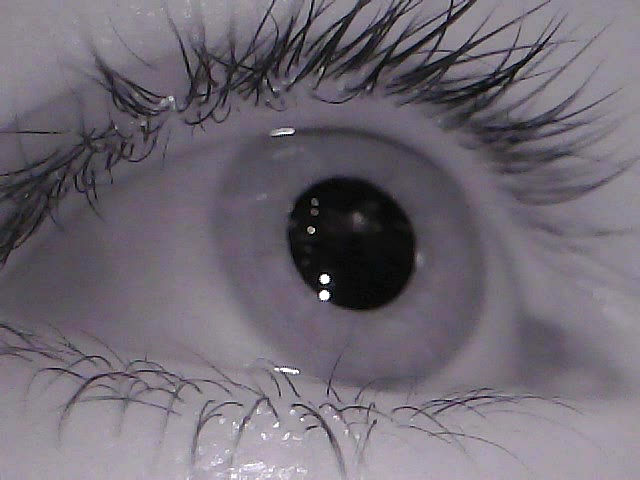
\includegraphics[width=.9\linewidth]{plots/eye_dataset/eye1.png}

      \label{fig:ds1}
    \end{subfigure}%
    \begin{subfigure}{.30\textwidth}
      \centering
      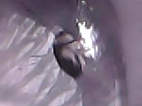
\includegraphics[width=.9\linewidth]{plots/eye_dataset/eye2.png}

      \label{fig:ds2}
    \end{subfigure}%
    \begin{subfigure}{.30\textwidth}
      \centering
      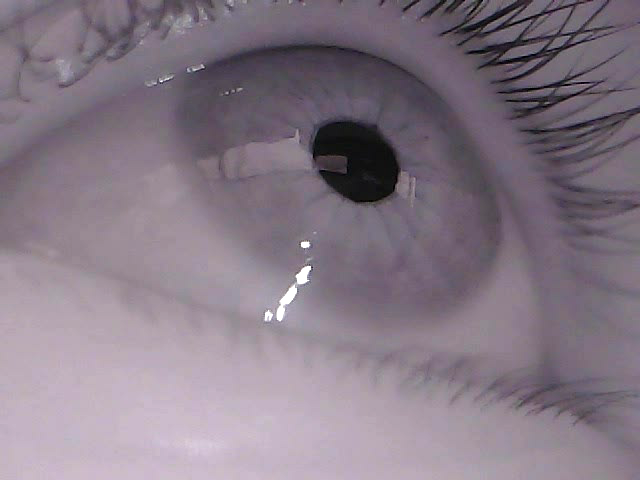
\includegraphics[width=.9\linewidth]{plots/eye_dataset/eye3.png}

      \label{fig:ds3}
    \end{subfigure}
    \caption{three example frames from the LPW data set.}
    \label{fig:example_frame}
    \end{figure}

    \subsection{Procedure}
    The participants were asked to look at a moving red ball as it moved around. The recording location was randomly picked and was in and around several buildings. Each location was chosen only once. 

    
\chapter{Theory}
\section{General Definitions}
This chapter discusses commonly used algorithms in image processing for edge detection, identifying areas of interest and applying them to pupil detection. At first, the algorithms will be discussed and analyzed on possible use cases, individual strengths and weaknesses. The algorithms use the same preprocessed images from the LPW data, so it is possible to showcase and compare the results. Even though different algorithms are used, the general approach for pupil detection can be summarized by finding the region of interest (ROI), then finding the pupil contour and finally approximating the pupil with an ellipse. Depending on the algorithm, the steps are sometimes extended or even combined. This chapter also discusses the possible combinations of algorithms. 

\subsection{Fundamental notation}\label{subsec:funda}
Throughout this thesis, the following notations are used to describe the algorithms.
The image with intensity level $I$ is a function:

$f(x,y): \mathbb{\mathbb{N_0} }^2 \rightarrow \mathbb{\mathbb{N_0}}$, where $f(x,y)$ is the intensity $I \in $ [$0,255$] at position $(x,y)$

In image processing, the coordinate system is defined differently than in mathematics. The origin is in the upper left corner and the x-axis points vertically down. The y-axis points horizontally to the right. This is shown in figure \ref{fig:coordsystem}.

\begin{figure}[h]
    \centering

\begin{tikzpicture}[x=0.3cm,y=-0.3cm]
    
    % Draw the x-axis
    \draw[->,thick] (0,8) -- (0,0) -- (8,0) node[below] {y};
    % Draw the y-axis
    \draw[->,thick] (0,0) -- (0,8) node[left] {x};
    % Label the origin
    \node at (0,0) [left] {0};
    \node at (0,0) [above] {0};
    \foreach \x in {1,2,...,7}
    \draw[gray, very thin] (\x,0) -- (\x,7);
  \foreach \y in {1,2,...,7}
    \draw[gray, very thin] (0,\y) -- (7,\y);
  \end{tikzpicture}

    \caption{Coordinate system used in image processing.}
    \label{fig:coordsystem}
\end{figure}

Also important to note is that the image is a discrete function: Therefore, each intensity value $I$ comes with a quantization error. The quantization error is also present when using an algorithm on the image's intensity values or position $(x,y)$. So it is not possible to have an exact result, it is always an approximation of the real result.

\subsection{Relationship between pixels}
Another important theory in this thesis will be based on the relationship between pixels. In this subsection, the terms \textbf{neighborhood}, \textbf{adjacency}, \textbf{connectivity}, \textbf{region} and \textbf{boundaries} will be introduced and visualized so that they can be used in the following chapters. 

\subsubsection{Neighborhood}
A pixel $P$ at location $(x,y)$ has two vertical neighbor pixels and two horizontal neighbor pixels in a 2D image. These neighbors are defined as $N_4(P)$ with coordinates: 
\begin{equation}
        N_4(P) = \{(x,y+1),(x,y-1),(x+1,y),(x-1,y)\}
\end{equation}
A pixel $P$ at location $(x,y)$ has four diagonal neighbor pixels in a 2D image. These neighbors are defined as $N_D(P)$ with coordinates:
\begin{equation}
    N_D(P) = \{(x+1,y+1),(x+1,y-1),(x-1,y+1),(x-1,y-1)\}
\end{equation}

Combining the neighbors from $N_4(P)$ and $N_D(P)$ results in the 8-neighborhood $N_8(P)$ of pixel $P$:
\begin{equation}
    N_8(P) = N_4(P) \cup N_D(P)
\end{equation}

Those three different types of neighbors are visualized in figure \ref{fig:neighborhoods}.

    \begin{figure}[ht]
        \centering
        \begin{subfigure}[b]{0.23\textwidth}
            \centering
            \begin{tikzpicture}[scale=0.6]
                \draw (0,0) grid (3,3);
                \filldraw[fill=orange!20] (1,0) rectangle (2,1);
                \filldraw[fill=orange!20] (1,2) rectangle (2,3);
                \filldraw[fill=orange!20] (0,1) rectangle (1,2);
                \filldraw[fill=orange!20] (2,1) rectangle (3,2);
                \filldraw[fill=black!90] (1,1) rectangle (2,2);
                \node[white] at (1.5,1.5) {P};
            \end{tikzpicture}
            \caption{$N_4(P)$}
            \label{fig:n_4}
        \end{subfigure}%
        \begin{subfigure}[b]{0.23\textwidth}
            \centering
            \begin{tikzpicture}[scale=0.6]
                \draw (0,0) grid (3,3);
                \filldraw[fill=blue!20] (0,3) rectangle (1,2);
                \filldraw[fill=blue!20] (2,0) rectangle (3,1);
                \filldraw[fill=blue!20] (0,0) rectangle (1,1);
                \filldraw[fill=blue!20] (2,2) rectangle (3,3);
                \filldraw[fill=black!90] (1,1) rectangle (2,2);
                \node[white] at (1.5,1.5) {P};
            \end{tikzpicture}
            \caption{$N_D(P)$}
            \label{fig:n_d}
        \end{subfigure}%
        \begin{subfigure}[b]{0.23\textwidth}
            \centering
            \begin{tikzpicture}[scale=0.6]
                \draw (0,0) grid (3,3);
                \filldraw[fill=blue!20] (0,3) rectangle (1,2);
                \filldraw[fill=blue!20] (2,0) rectangle (3,1);
                \filldraw[fill=blue!20] (0,0) rectangle (1,1);
                \filldraw[fill=blue!20] (2,2) rectangle (3,3);
                \filldraw[fill=orange!20] (1,0) rectangle (2,1);
                \filldraw[fill=orange!20] (1,2) rectangle (2,3);
                \filldraw[fill=orange!20] (0,1) rectangle (1,2);
                \filldraw[fill=orange!20] (2,1) rectangle (3,2);
                \filldraw[fill=black!90] (1,1) rectangle (2,2);

                \node[white] at (1.5,1.5) {P};
            \end{tikzpicture}
            \caption{$N_8(P)$}
            \label{fig:n_8}
        \end{subfigure}%
        \caption{3 different neighborhoods of pixel $P$ at location $(x,y)$.}
        \label{fig:neighborhoods}
    \end{figure}


\subsubsection{Adjacency} There are three types of adjacent pixels in a 2D image. Let $V$ be the set of intensity values used to define adjacency. Depending on the intensity range of the image, it is possible to define different subsets of $V$, containing the intensity values considered adjacent if they are present in the neighborhood. In a binary image, $V$ is often defined as $V$ = $\{1\}$, where $0$ stands for background and $1$ for foreground (This can also be considered a binary mask). In a grayscale image, $V$ can be defined as any subset of the intensity range.

To keep it simple, the following explanations uses a binary image with $V$ = $\{1\}$. Let's define $P$ as a pixel at location $(x,y)$ and $Q$ as a pixel at location $(x',y')$. $P$ and $Q$ are considered adjacent if $Q$ is in the neighborhood of $P$ and $f(Q)$ is $\in V$. These are the three adjacency types:

\begin{itemize}
    \item 4-adjacency, if $Q_i \in N_4(P) and f(Q_i) \in  V$: The pixels directly above, below, left and right of the pixel. 
    \item 8-adjacency, if $Q_i \in N_8(P) and f(Q_i) \in  V$: The pixels directly above, below, left, right and the pixels diagonally adjacent to the pixel.
\end{itemize}
These two adjacency types are visualized in figure \ref{fig:adjacency}.
\begin{equation*}
    \bullet \text{ m-adjacency} \begin{cases}
   \text{if } Q \in N_4(P) \text{ and } f(Q) \in  V \\
    Q \in N_D(P) \text{ and } N_D(P)  \cap N_4(Q) \text{ has no intensities} \in  V
    \end{cases}
    \end{equation*}


    \begin{figure}[ht]
        \centering
        \begin{subfigure}{0.40\textwidth}
            \centering
            \begin{tikzpicture}[scale=0.6]
                \draw (0,0) grid (3,3);
                \filldraw[fill=orange!20] (1,0) rectangle (2,1);
                \filldraw[fill=orange!20] (1,2) rectangle (2,3);
                \filldraw[fill=orange!20] (0,1) rectangle (1,2);
                \filldraw[fill=orange!20] (2,1) rectangle (3,2);
                \filldraw[fill=black!90] (1,1) rectangle (2,2);


                \node[white] at (1.5,1.5) {$P$};
                \node at (1.5,2.5) {$Q_1$};
                \node at (0.5,1.5) {$Q_2$};
                \node at (2.5,1.5) {$Q_3$};
                \node at (1.5,0.5) {$Q_4$};




            \end{tikzpicture}
            \caption{4-adjacency}
            \label{fig:a_4}
        \end{subfigure}%
        \begin{subfigure}{0.40\textwidth}
            \centering
            \begin{tikzpicture}[scale=0.6]
                \draw (0,0) grid (3,3);
                \filldraw[fill=blue!20] (0,3) rectangle (1,2);
                \filldraw[fill=blue!20] (2,0) rectangle (3,1);
                \filldraw[fill=blue!20] (0,0) rectangle (1,1);
                \filldraw[fill=blue!20] (2,2) rectangle (3,3);
                \filldraw[fill=blue!20] (1,0) rectangle (2,1);
                \filldraw[fill=blue!20] (1,2) rectangle (2,3);
                \filldraw[fill=blue!20] (0,1) rectangle (1,2);
                \filldraw[fill=blue!20] (2,1) rectangle (3,2);
                \filldraw[fill=black!90] (1,1) rectangle (2,2);
                \node[white] at (1.5,1.5) {$P$};
                \node at (0.5,0.5) {$Q_6$};
                \node at (1.5,0.5) {$Q_7$};
                \node at (2.5,0.5) {$Q_8$};
                \node at (0.5,1.5) {$Q_4$};
                \node at (2.5,1.5) {$Q_5$};
                \node at (0.5,2.5) {$Q_1$};
                \node at (1.5,2.5) {$Q_2$};
                \node at (2.5,2.5) {$Q_3$};
            \end{tikzpicture}
            \caption{$8-adjacency$}
            \label{fig:a_8}
        \end{subfigure}%

        \caption{3 different neighborhoods of pixel $P$ at location $(x,y)$.}
        \label{fig:adjacency}
    \end{figure}
\subsubsection{Connectivity}
The connectivity of point $P$ is a set of points that can be reached in $n$ steps with a given adjacency type and intensity set $V$. If point $P$ is connected with $Q$, then there exists a path (or curve) from $P$ to $Q$, that consists of a sequence of distinct pixels with coordinates:
\begin{equation*}
    (x_0,y_0),(x_1,y_1),...,(x_n,y_n), 
\end{equation*}
Where $n$ is the length of the path. If the path is closed then $(x_0,y_0) = (x_n,y_n)$
\subsubsection{Region}
Let's define $R$ as a subset of pixels in an image. $R$ is a region if all points $\in R$ are a connected set, meaning that all points in $R$ are connected with each other and therefore form a region. This does not mean that the path connecting all points is closed. Two regions can be adjacent to each other, if their union again forms a connected set. 

\subsubsection{Boundary}
The outer boundary of a region $R$ is the set of pixels not in $R$ adjacent to pixels in $R$. In the definition of a boundary, the adjacency type is of importance. As a rule of thumb the 8-adjacency is used to define the boundary. One critical property of the outer boundary is, that it is a closed path. The inner boundary is the set of pixels in $R$ that are 8-adjacent to at least one pixel $\notin  R$. In figure \ref{fig:regbond} it can be seen that the outer boundary is a closed path, whereas the inner boundary, in this example identical to the region is not a closed path.

\begin{figure}[ht]
    \centering
    \begin{subfigure}{0.40\textwidth}
        \centering
        \begin{tikzpicture}
            \matrix [matrix of nodes, nodes in empty cells, nodes={minimum width=1.5em, minimum height=1.5em, draw, thick, anchor=center}, column sep=-\pgflinewidth, row sep=-\pgflinewidth] (M)
            {
                |[fill=gray!20]| & |[fill=gray!20]| & |[fill=gray!20]| & |[fill=gray!20]| & |[fill=gray!20]| & |[fill=gray!20]| & |[fill=gray!20]| \\
                |[fill=gray!20]| & |[fill=gray!20]| & |[fill=gray!20]| & |[fill=red!20]|1 & |[fill=red!20]|1 & |[fill=gray!20]| & |[fill=gray!20]| \\
                |[fill=gray!20]| & |[fill=gray!20]| & |[fill=gray!20]| & |[fill=gray!20]| & |[fill=red!20]|1 & |[fill=red!20]|1 & |[fill=gray!20]| \\
                |[fill=gray!20]| & |[fill=gray!20]| & |[fill=gray!20]| & |[fill=gray!20]| & |[fill=gray!20]| & |[fill=red!20]|1 & |[fill=gray!20]| \\
                |[fill=gray!20]| & |[fill=red!20]|1 & |[fill=gray!20]| & |[fill=gray!20]| & |[fill=red!20]|1 & |[fill=red!20]|1 & |[fill=gray!20]| \\
                |[fill=gray!20]| & |[fill=red!20]|1 & |[fill=red!20]|1 & |[fill=red!20]|1 & |[fill=red!20]|1 & |[fill=gray!20]| & |[fill=gray!20]| \\
                |[fill=gray!20]| & |[fill=gray!20]| & |[fill=gray!20]| & |[fill=gray!20]| & |[fill=gray!20]| & |[fill=gray!20]| & |[fill=gray!20]| \\
            };
            
            \draw [thick] (M-1-1.north west) rectangle (M-7-7.south east);
        \end{tikzpicture}
        
        
            
        \caption{region $R$}
        \label{fig:region}
    \end{subfigure}%
    \begin{subfigure}{0.40\textwidth}
        \centering
        \begin{tikzpicture}
            \matrix [matrix of nodes, nodes in empty cells, nodes={minimum width=1.5em, minimum height=1.5em, draw, thick, anchor=center}, column sep=-\pgflinewidth, row sep=-\pgflinewidth] (M)
            {
                |[fill=gray!20]| & |[fill=gray!20]| & |[fill=red!20]| & |[fill=red!20]| & |[fill=red!20]| & |[fill=red!20]| & |[fill=gray!20]| \\
                |[fill=gray!20]| & |[fill=gray!20]| & |[fill=red!20]| & 1 & 1 & |[fill=red!20]| & |[fill=red!20]| \\
                |[fill=gray!20]| & |[fill=gray!20]| & |[fill=red!20]| & |[fill=red!20]| & 1 & 1 & |[fill=red!20]| \\
                |[fill=red!20]| & |[fill=red!20]|& |[fill=red!20]| & |[fill=red!20]| & |[fill=red!20]| & 1 & |[fill=red!20]| \\
                |[fill=red!20]| & 1 & |[fill=red!20]| & |[fill=red!20]| & 1 & 1 & |[fill=red!20]| \\
                |[fill=red!20]| & 1 & 1 & 1 & 1 & |[fill=red!20]| & |[fill=red!20]| \\
                |[fill=red!20]| & |[fill=red!20]| & |[fill=red!20]| & |[fill=red!20]| & |[fill=red!20]| & |[fill=red!20]| & |[fill=gray!20]| \\
            };
        
            \draw [thick] (M-1-1.north west) rectangle (M-7-7.south east);
        \end{tikzpicture}
        
        \caption{outer boundary (8-adjacent)}
        \label{fig:boundary}
    \end{subfigure}%
    \caption{Region and outer border.}
    \label{fig:regbond}
\end{figure}
\subsection{Preprocessing}
The preprocessing must be defined first to compare the different approaches for pupil detection. The idea behind this step is to create a common ground for narrowing the deviation of the images down so that the algorithms can recreate the same result for different images.

\subsubsection{Converting to grayscale}
As presented in the previous chapter, the iris is the only colorful part of the eye. However, the color itself is of no interest for the detection. Therefore the frames are first converted to grayscale. 
In this thesis the grayscale images have the intensity values $I \in [0,255]$ and the image size is depending on the scaling as shown in table \ref{tab:resoluiton}. The scaling is done to reduce the computational cost of the algorithm. 

\begin{table}[h]
    \centering 
    \begin{minipage}{0.7\textwidth}
      \centering
      \begin{tabular}{|c|c|c|}
        \hline
        Scaling &  Shape & numpy array type \\
        \hline
        100\% & 640x480& uint8 \\
        50\% & 320x240 & uint8 \\
        25\% & 160x120 & uint8 \\
        12.5\% & 80x60 & uint8 \\
        6.25\% & 40x30 & uint8 \\
        \hline
      \end{tabular}
      \caption{Scaling of the frames used in this thesis.}
      \label{tab:resoluiton}
    \end{minipage}\hfill
\end{table}

It is important to note that these resolutions are congruent with the LPW paper \cite{zhang_max-planck-institut_2016}. This is important for the comparison of the results.
When scaling an image, an interpolation is alway done to find the best approximation for the new intensity value $I$ at location $(x,y)$. 

The interpolation used in this thesis is the bilinear interpolation\cite{gonzalez_bilinear_2018}. This is a linear interpolation in the x and y-axis of the intensity values and solves equation \ref{eq:bilinear}.
\begin{equation}
    v(x,y) = ax + by + cxy + d 
    \label{eq:bilinear}
\end{equation}

Let $Q_{11}=(x_1,y_1)$, $Q_{12}=(x_1,y_2)$, $Q_{21}=(x_2,y_1)$ and $Q_{22}=(x_2,y_2)$ be the four surrounding points. The intensity value $v$ at $(x,y)$ is calculated by equation \ref{eq:bilinear}.The point P at $(x,y)$ is the point of interest. The visualization of the bilinear interpolation is shown in figure \ref{fig:blinearInterpolation}.
\begin{figure}[h]
    \centering
    \begin{tikzpicture}[x=0.5cm,y=-0.5cm]
    
    % Draw the x-axis
    \draw[->,thick] (0,8) -- (0,0) -- (8,0) node[below] {y};
    % Draw the y-axis
    \draw[->,thick] (0,0) -- (0,8) node[left] {x};
    % Label the origin
    \node at (0,0) [left] {0};
    \node at (0,0) [above] {0};
    \foreach \x in {2,4,7}
    \draw[gray, very thin] (\x,0) -- (\x,7);
  \foreach \y in {2,4,7}
    \draw[gray, very thin] (0,\y) -- (7,\y);

    \foreach \Point/\PointLabel in {(7,4)/R_2,(2,4)/R_1}
    \draw[fill=red] \Point circle (0.3) node[above right] {$\PointLabel$};

    \foreach \Point/\PointLabel in {(2,2)/Q_{11}, (7,2)/Q_{12}, (2,7)/Q_{21}, (7,7)/Q_{22}}
    \draw[fill=black] \Point circle (0.3) node[above right] {$\PointLabel$};

    \foreach \Point/\PointLabel in {(4,4)/P }
    \draw[fill=blue] \Point circle (0.35) node[above right] {$\PointLabel$};

  \end{tikzpicture}

    \caption{Bilinear interpolation.}
    \label{fig:blinearInterpolation}
\end{figure}

First the intensity values $I_1 = f(R_1)$ and $I_2 = f(R_2)$ are calculated. $f(R_1)$ is the linear interpolation between $Q_{11}$ and $Q_{21}$
\begin{equation}
    f(R_{1}) \approx \frac{x_{2}-x}{x_{2}-x_{1}}f(Q_{11})+\frac{x-x_{1}}{x_{2}-x_{1}}f(Q_{21}) = R_{1}(x,y_{1})
\end{equation}
 $f(R_2)$ is the linear interpolation between $Q_{12}$ and $Q_{22}$.
 \begin{equation}
    f(R_{2}) \approx \frac{x_{2}-x}{x_{2}-x_{1}}f(Q_{12})+\frac{x-x_{1}}{x_{2}-x_{1}}f(Q_{22}) = R_{2}(x,y_{2})
\end{equation}
 Then the intensity value $I = f(P)$ at $P$ is calculated by the linear interpolation between $R_1$ and $R_2$. 
\begin{equation}
    f(P) \approx \frac{y_{2}-y}{y_{2}-y_{1}}f(R_{1})+ \frac{y-y_{1}}{y_{2}-y_{1}}f(R_{2}) = v(x,y)
\end{equation}
Therefore $f(P) = v(x,y)$ is the intensity value at $P$ calculated with the bilinear interpolation of $Q_{11}$, $Q_{12}$, $Q_{21}$ and $Q_{22}$ at $P$.



\subsubsection{Histogram equalization }
Another vital aspect of preprocessing the frames is using Histogram equalization \cite{noauthor_opencv_2015}. Histogram equalization has the effect of increasing the contrast of the image. This thesis uses Contras Limited Adaptive Histogram Equalization (CLAHE). CLAHE is a histogram equalization method that has the benefit that it is adaptive to the local contrast of the image. Local contrast equalization is very useful if the contrast of the image is not uniform in all regions of the image. Using Histogram Equalization adds additional noise to the image. The additional noise can be dealt with using a low pass filter, like a Gaussian filter for example, to minimize the noise. 

 Using a standard Histogram Equalization approach would lead to a loss of information in the region around the pupil and the iris because this is the region with the highest contrast already. Therefore, more noise would be added to the pupil and iris region. The CLAHE method splits the image into smaller blocks called "tiles". CLAHE then calculates the histogram equalization on each block individually without losing the same amount of information in the pupil region compared to the standard histogram equalization. The CLAHE method is applied to the frames after they are converted to grayscale. The result of this step is shown in figure \ref{fig:clahe}. 

\begin{figure}[h]
    \centering
    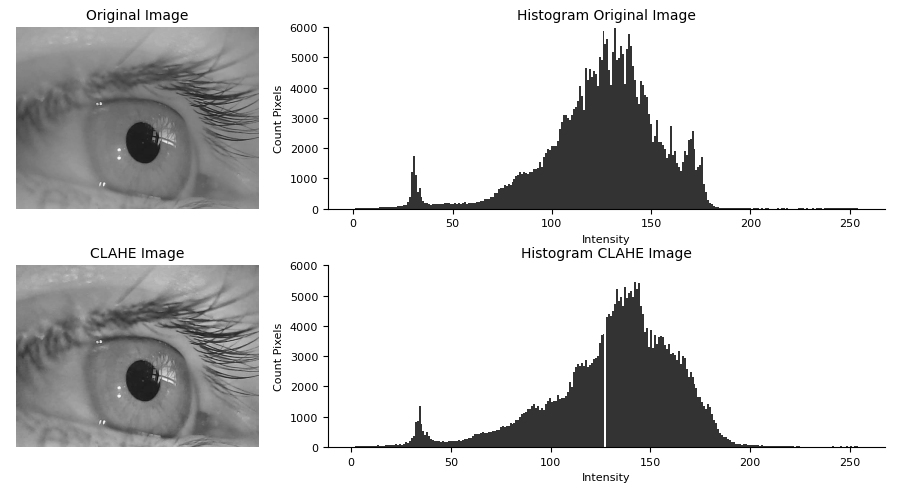
\includegraphics[width=1\textwidth]{plots/clahe.png}
    \caption{Example of CLAHE an its effect on the histogram.}
    \label{fig:clahe}
\end{figure}

\section{Edge Detection}
The main goal behind edge detection is to find edges in the image. An edge is defined as a region with high contrast to its surrounding pixels, in other words, a rapid change of intensity in a small area. Edge detection is helpful to filter the image for possible pupil contours. The edge detection analysis is based on a gradient calculation. There are different methods to calculate the gradient of an image. One of the most popular methods is the Sobel operator, which uses the first differential of the intensity change in the image. The Laplacian operator is another method that uses the second differential of the intensity change in the image. In this thesis the Sobel operator is used to calculate the gradient of the image. 
After calculating the gradient, Canny edge detection is used to refine the edges. Canny edge detection is a multi-step algorithm that uses hysteresis thresholding to filter the edges. The edge detection result is a one pixel thick binary edge map.  These edges are now possible candidates for the pupil contour and need additional processing steps to find the pupil contour. 
\subsection{Sobel Operators}
The Sobel Operators \cite{gonzalez_sharpening_2018} is commonly used for edge detection. It is a gradient calculation that uses two 3x3 differential kernels to calculate the gradient of the image. The Sobel gradient is calculated in the x and y direction with their corresponding kernels $k_x$ and $k_y$, and the kernels are defined as:
\begin{center}
    \begin{minipage}{0.44\textwidth}
        \begin{equation}
            k_x = \begin{bmatrix}
                -1 & 0 & +1 \\
                -2 & 0 & +2 \\
                -1 & 0 & +1
            \end{bmatrix} 
        \end{equation}
    \end{minipage}
    \hfill
    \begin{minipage}{0.44\textwidth}
        \begin{equation}
            k_y = \begin{bmatrix}
                -1 & -2 & -1 \\
                0 & 0 & 0 \\
                +1 & +2 & +1
            \end{bmatrix} 
        \end{equation}
         
    \end{minipage}
    
\end{center}
     The gradient vector is $\nabla f(x,y) = [G_x, G_y]^T$  and is calculated by convolving the image $f(x,y)$ with the Sobel kernels $k_x$, $k_y$ and $a,b = 1$.
     \begin{align}
        G_x(x,y) & = f(x,y) * k_x  = \sum_{s=-a}^{a} \sum_{t=-b}^{b} k_x(s,t) f(x+s,y+t) \\
        G_y(x,y) & = f(x,y) * k_y  = \sum_{s=-a}^{a} \sum_{t=-b}^{b} k_y(s,t) f(x+s,y+t)
    \end{align}
     
    $G_x(x,y) = \partial f/ \partial x$ and $G_y(x,y)= \partial f/ \partial y$ are the gradients in x and y direction and the total gradient magnitude $G$ of the gradient vector is calculated with the euclidean norm: 
    \begin{equation}
        G = \sqrt{G_x^2 + G_y^2}
        \label{eq:gradientmagnitude}
    \end{equation} 
    the orientation $\theta$ of the gradient is :
    \begin{equation}
        \theta = \arctan2{\frac{G_y}{G_x}}
        \label{eq:gradientdirection}
    \end{equation}
    The result of the gradient calculation can be seen here:
    \begin{figure}[ht]
        \centering
        % First row: 3 images
        \begin{subfigure}{.33\textwidth}
          \centering
          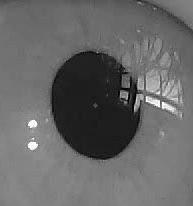
\includegraphics[width=.9\linewidth]{plots/eye_dataset/roi.png}
          \caption{Image of ROI}
          \label{fig:roig}
        \end{subfigure}%
        \begin{subfigure}{.33\textwidth}
          \centering
          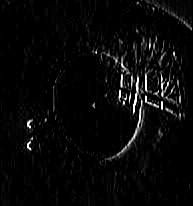
\includegraphics[width=.9\linewidth]{plots/eye_dataset/sx.png}
          \caption{Gradient in x \textbf{$G_{x}$}}
          \label{fig:sx}
        \end{subfigure}%
        \begin{subfigure}{.33\textwidth}
          \centering
          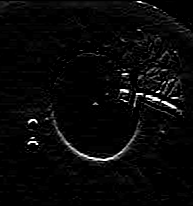
\includegraphics[width=.9\linewidth]{plots/eye_dataset/sy.png}
          \caption{Gradient in y \textbf{$G_{y}$}}
          \label{fig:sy}
        \end{subfigure}
        % Second row: 2 images
        \begin{subfigure}{.33\textwidth}
          \centering
          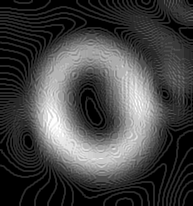
\includegraphics[width=.9\linewidth]{plots/eye_dataset/mag.png}
          \caption{Magnitude \textbf{$G$}}
          \label{fig:mag}
        \end{subfigure}%
        \begin{subfigure}{.33\textwidth}
          \centering
          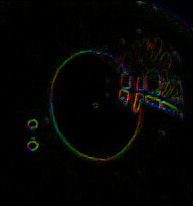
\includegraphics[width=.9\linewidth]{plots/eye_dataset/direction.png}
          \caption{Orientation \textbf{$\theta$}}
          \label{fig:orientation}
        \end{subfigure}
        \caption{Plot of gradient characteristics of the ROI.}
        \label{fig:gradient}
        \end{figure}
    Important to note is that figure \ref{fig:mag} and figure \ref{fig:orientation} are the results of a strong gaussian blurred initial image. 
    \subsection{Canny Edge Detection } 
    The Canny Edge Detection \cite{gonzalez_canny_2018} calculates single edge points from the gradient vector image.  
    Canny edge detection can be summarized in four steps: 
    \begin{enumerate}
        \item Noise reduction, smooth the image with a Gaussian filter
        \item Compute the gradient magnitude and direction
        \item Non-maximum suppression to the gradient magnitude image
        \item Use double thresholding and connectivity analysis to detect and link edges
    \end{enumerate}
\textbf{Step 1: Noise reduction} \\
The first step is to reduce noise from the input image. This is done by convolving the image with a low pass filter. For this task a Gaussian filter is used. The Gaussian filter is:
\begin{equation}
    f_{filter}(x,y) = \frac{1}{2\pi\sigma^2}e^{-\frac{x^2+y^2}{2\sigma^2}}
\end{equation}
The Gaussian filter is then convolved with the image to smooth the image. 
\begin{equation}
    f_{smoothed}(x,y) = f(x,y) * f_{filter}(x,y)
\end{equation} 

\textbf{Step 2: Compute the gradient magnitude and direction} \\
The gradient magnitude $G$ is calculated with equation \ref{eq:gradientmagnitude} and the gradient direction $\theta$ is calculated with equation \ref{eq:gradientdirection}.

\textbf{Step 3: Non-maximum suppression} \\
The non-maximum suppression is used to thin the edges out so the edges are only one pixel wide. This can be achieved with a loop iterating over all edge pixels and individually checking if the current pixel is the local maximum in the gradient vector's direction $\pm \theta$. If the pixel indeed is the local maximum, the pixel is kept, otherwise it is set to zero. Because as already described in \ref{subsec:funda} the coordinate system is defined differently. The gradient direction $\theta$ is in reference to the $x$ axis.

\begin{figure}[h]
    \centering
        \begin{tikzpicture}[rotate=-90, scale= 0.5]
            % Draw the coordinate axes
            \draw[->] (-3,0) -- (3,0) node[right] {$x$};
            \draw[->] (0,-3) -- (0,3) node[above] {$y$};
            % Draw the first line
            \draw (2,0) arc (0:31:2)node[above right] {$\theta$};
            \draw[->,red,thick] (0,0) -- (2.5,1.5)node[right] {Gradient Vector};
            % Draw the angle marker
        
        ;
            % Draw the second line
            \draw[blue,thick] (1.5,-2.5) -- (-1.5,2.5)node[above right] {$Edge$};
            % Draw the origin
            \filldraw[black] (0,0) circle (2pt);
        \end{tikzpicture}
        \caption{Definition of the gradient direction}
        \label{fig:Definition_grad}
\end{figure}
Because an image is quantized, this also means that $\theta$ needs to be quantized in four directions to evaluate their neighbors. 

\begin{figure}[h]
    \centering
\begin{tikzpicture}[x=1cm,y=1cm]
    % Draw the grid
    \draw (0,0) grid (3,3);
     % Draw unit circle around grid

    % Fill the center pixel with light gray
    \filldraw[fill=blue!20] (0,0) rectangle (1,1);
    \filldraw[fill=blue!20] (2,2) rectangle (3,3);
    \filldraw[fill=orange!20] (0,1) rectangle (1,2);
    \filldraw[fill=orange!20] (2,1) rectangle (3,2);
    \filldraw[fill=red!20] (0,3) rectangle (1,2);
    \filldraw[fill=red!20] (2,0) rectangle (3,1);
    \filldraw[fill=green!20] (1,0) rectangle (2,1);
    \filldraw[fill=green!20] (1,2) rectangle (2,3);
    \filldraw[fill=black!60] (1,1) rectangle (2,2);


    \draw (1.5, 1.5) circle [radius=2.12];
    % Mark angles in 45° steps
    \foreach \ang in {157.5,112.5,67.5,22.5,-22.5,-67.5,-112.5,-157.5} {
        \draw (\ang-90:3.5) ++(1.5,1.5) node [fill=white] {$\ang^\circ$};
        \draw (\ang-90:3) ++(1.5,1.5) -- (1.5,1.5) ;

    }
    \foreach \ang in {0,180} {
        %\draw[thick,green] (\ang-90:2.3) ++(1.5,1.5) -- (1.5,1.5) ;
        \draw (\ang-90:2.1) ++(1.5,1.5) node [fill=green!20] {$\ang^\circ$};

    }

    \foreach \ang in {-45,135} {
        %\draw[thick,blue] (\ang-90:2.3) ++(1.5,1.5) -- (1.5,1.5) ;
        \draw (\ang-90:2.1) ++(1.5,1.5) node [fill=blue!20] {$\ang^\circ$};


    }
    \foreach \ang in {-90,90} {
        %\draw[thick,orange] (\ang-90:2.3) ++(1.5,1.5) -- (1.5,1.5) ;
        \draw (\ang-90:2.1) ++(1.5,1.5) node [fill=orange!20] {$\ang^\circ$};


    }
    \foreach \ang in {45,-135} {
        %\draw[thick,red] (\ang-90:2.3) ++(1.5,1.5) -- (1.5,1.5) ;
        \draw (\ang-90:2.1) ++(1.5,1.5) node [fill=red!20] {$\ang^\circ$};


    }

         % Add a tick at 45 degrees

\end{tikzpicture}
  \caption{Quantization of the gradient direction}
  \label{fig:non_max}
\end{figure}
This leads to following quantizations: 
\begin{equation}
    \theta_q = \begin{cases}
    90, & \text{if } 67.5^\circ < \theta \leq 112.5^\circ \, \vee \, -112.5^\circ < \theta \leq -67.5^\circ \\
    -45^\circ, &\text{if }22.5^\circ < \theta \leq 67.5^\circ \, \vee \, -157.5^\circ < \theta \leq -112.5^\circ \\
    +45^\circ, &\text{if }112.5^\circ <\theta \leq 157.5^\circ \, \vee \, -67.5^\circ < \theta \leq -22.5^\circ \\
    0^\circ, &\text{if }-22.5^\circ <\theta \leq 22.5^\circ \, \vee \, -157.5^\circ < \theta \leq 157.5^\circ \\
\end{cases} 
\label{eq:quantization_d}
\end{equation}
It is important to note that two neighboring pixels are used to evaluate the gradient magnitude maximum. This is shown in figure \ref{fig:non_max} and \ref{fig:neighbors}.
Suppose the maximum gradient magnitude is at the current pixel at $(x,y)$, meaning it is a local maximum in the previously defined neighborhood with respect to the gradient direction, the value of the pixel is written into $g_n(x,y)$. Otherwise, it is set to zero $g_n(x,y) = 0$. $g_n(x,y)$ is the non-maximum suppressed edge image. Therefore $g_n(x,y)$ contains only the thinned edges.  

\begin{figure}[ht]
    \centering
    \begin{subfigure}[b]{0.23\textwidth}
        \centering
        \begin{tikzpicture}[scale=0.6]
            \draw (0,0) grid (3,3);
            \filldraw[fill=orange!20] (0,1) rectangle (1,2);
            \filldraw[fill=orange!20] (2,1) rectangle (3,2);
            \filldraw[fill=black!60] (1,1) rectangle (2,2);
        \end{tikzpicture}
        \caption{Neighbors: 90°}
        \label{fig:n90}
    \end{subfigure}%
    \begin{subfigure}[b]{0.23\textwidth}
        \centering
        \begin{tikzpicture}[scale=0.6]
            \draw (0,0) grid (3,3);
            \filldraw[fill=red!20] (0,3) rectangle (1,2);
            \filldraw[fill=red!20] (2,0) rectangle (3,1);
            \filldraw[fill=black!60] (1,1) rectangle (2,2);
        \end{tikzpicture}
        \caption{Neighbors: 45°}
        \label{fig:n45}
    \end{subfigure}%
    \begin{subfigure}[b]{0.23\textwidth}
        \centering
        \begin{tikzpicture}[scale=0.6]
            \draw (0,0) grid (3,3);
            \filldraw[fill=blue!20] (0,0) rectangle (1,1);
            \filldraw[fill=blue!20] (2,2) rectangle (3,3);
            \filldraw[fill=black!60] (1,1) rectangle (2,2);
        \end{tikzpicture}
        \caption{Neighbors: -45°}
        \label{fig:nn45}
    \end{subfigure}%
    \begin{subfigure}[b]{0.23\textwidth}
        \centering
        \begin{tikzpicture}[scale=0.6]
            \draw (0,0) grid (3,3);
            \filldraw[fill=green!20] (1,0) rectangle (2,1);
            \filldraw[fill=green!20] (1,2) rectangle (2,3);
            \filldraw[fill=black!60] (1,1) rectangle (2,2);
        \end{tikzpicture}
        \caption{Neighbors: 0°}
        \label{fig:n0}
    \end{subfigure}
    \caption{The gradient magnitude is evaluated in the direction of the gradient.}
    \label{fig:neighbors}
\end{figure}

  

\textbf{Step 4: Double thresholding and connectivity analysis} \\
After Step 3, $g_n(x,y)$ still contains edges that can be thicker than one pixel. $g_n(x,y)$ is then thresholded with a high and a low threshold value (hysteresis thresholding), creating two images: 
\begin{equation}
    g_{low}(x,y) = \begin{cases}
    g_n(x,y), & \text{if } g_n(x,y) \geq T_{low} \\
    0, &\text{otherwise}
\end{cases}
\end{equation}
\begin{equation}
    g_{high}(x,y) = \begin{cases}
    g_n(x,y), & \text{if } g_n(x,y) \geq T_{high} \\
    0, &\text{otherwise}
\end{cases}
\end{equation}
Because two different thresholds are used, there is still an overlap between $g_{low}$ and $g_{high}$ edges. All non-zero pixels in $g_{high}$ are considered strong edge pixels. To find all weak edge pixels, the strong edge pixels are substracted from $g_{low}$. 
\begin{equation}
    g_{weak}(x,y) = g_{low}(x,y) - g_{high}(x,y)
\end{equation}
The remaining pixels are considered weak edge pixels.

The next step is to connect the weak edge pixels to the strong edge pixels. This is done by checking the 8-neighborhood of each strong edge pixel. If there is a weak edge pixel in the neighborhood, it is considered a strong edge pixel. This continues until no more weak edge pixels are found. The result is a binary image $g_{final}(x,y)$ containing connected edges. $g_{final}(x,y)$ still doesn't consists of one-pixel thick edges. 

An edge-thinning algorithm solves this problem and returns the wanted image with only one-pixel thick edges. Let's define the edges as set A and a structuring element as B. 
The equation for thinning is: 
\begin{equation}
    A \otimes   B = A - (A \circledast B)
\end{equation}
Where $\otimes$ is the thinning operator, $\circledast$ is the dilation operator.

\subsubsection{Results}
In a frame where the pupil region is clearly distinguishable from the rest, the Canny edge detector can be used to find the pupil boundary. But as soon as more noise to the pupil is added, the hysteresis thresholding becomes more tricky and the detection accuracy decreases immensely. Also it is not possible to differentiate between the eye leashes, eyebrows and the pupil. Therefore by using only the Canny edge detector, the pupil edges can not be found reliably and the algorithm itself is not adaptable to a great variety of environments. The problem with Canny edge detection is visualized in figure \ref{fig:canny_clear} and \ref{fig:canny_eyelid}.


\begin{figure}[ht]
    \centering
    \begin{subfigure}{.5\textwidth}
      \centering
      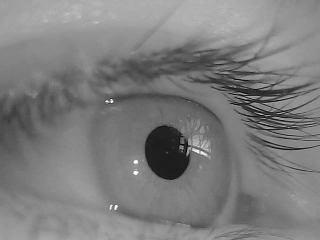
\includegraphics[width=.9\linewidth]{plots/orig_canny.png}
      \caption{Original image, scaling 0.5}
      \label{fig:orig_canny}
    \end{subfigure}%
    \begin{subfigure}{.5\textwidth}
      \centering
      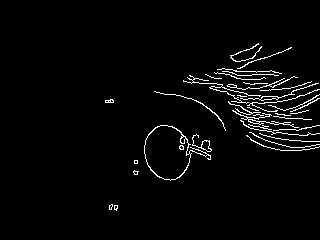
\includegraphics[width=.9\linewidth]{plots/canny.png}
      \caption{Clear pupil region, Canny edge detection}
      \label{fig:canny_region_clear}
    \end{subfigure}
    \caption{Canny edge detection on a clear pupil region}
    \label{fig:canny_clear}
\end{figure}

\begin{figure}[ht]
    \centering
    \begin{subfigure}{.5\textwidth}
      \centering
      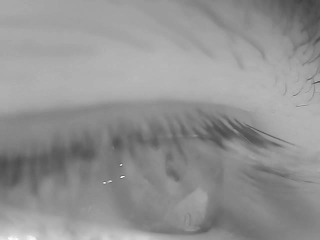
\includegraphics[width=.9\linewidth]{plots/orig_canny_eyelids.png}
      \caption{Original image, scaling 0.5}

    \end{subfigure}%
    \begin{subfigure}{.5\textwidth}
      \centering
      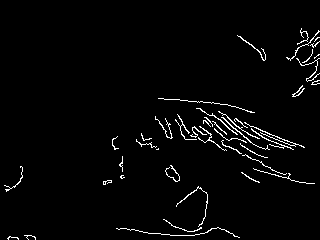
\includegraphics[width=.9\linewidth]{plots/canny_eyelids.png}
      \caption{Weak pupil region, Canny edge detection}

    \end{subfigure}
    \caption{Canny Edge detection on a frame with weak pupil region}
    \label{fig:canny_eyelid}
\end{figure}

\section{Haar-like feature detection }
\label{subsec:haar}
\subsection{Concept}
Haar-like features \cite{viola_rapid_2004} are based on the observation that objects have a particular local intensity variation in an image which can be useful for identifying objects. Haar-like features use the intensity variation and divide the image into rectangular regions and then calculate the difference between the sum of the pixel's intensity in the white and gray regions. An overview of the structure of features is given in \ref{fig:haar_features}.
\begin{figure}[h]
    \centering
    
    \begin{subfigure}{0.45\textwidth}
        \centering
        \begin{tikzpicture}[scale=0.8, transform shape]
            % Haar-like feature: Two-rectangle feature
            \draw[fill=gray] (0,0) rectangle (1,1);
            \draw[fill=white] (1,0) rectangle (2,1);
        \end{tikzpicture}
        \caption{Two-Rectangle Feature}
        \label{fig:haar_feature_1}
    \end{subfigure}
    \hfill
    \begin{subfigure}{0.45\textwidth}
        \centering
        \begin{tikzpicture}[scale=0.8, transform shape]
            % Haar-like feature: Three-rectangle feature
            \draw[fill=gray] (0,0) rectangle (1,1);
            \draw[fill=white] (1,0) rectangle (2,1);
            \draw[fill=gray] (2,0) rectangle (3,1);
        \end{tikzpicture}
        \caption{Three-Rectangle Feature}
        \label{fig:haar_feature_2}
    \end{subfigure}
    
    \vspace{1.5em}
    
    \begin{subfigure}{0.45\textwidth}
        \centering
        \begin{tikzpicture}[scale=0.8, transform shape]
            % Haar-like feature: Line feature (Horizontal)
            \draw[fill=gray] (0,0) rectangle (2,1);
            \draw[fill=white] (0,-1) rectangle (2,0);
        \end{tikzpicture}
        \caption{Horizontal Line Feature}
        \label{fig:haar_feature_3}
    \end{subfigure}
    \hfill
    \begin{subfigure}{0.45\textwidth}
        \centering
        \begin{tikzpicture}[scale=0.8, transform shape]
            % Haar-like feature: Four-rectangle feature
            \draw[fill=gray] (0,0) rectangle (1,1);
            \draw[fill=white] (1,0) rectangle (2,1);
            \draw[fill=gray] (0,1) rectangle (1,2);
            \draw[fill=white] (1,1) rectangle (2,2);
        \end{tikzpicture}
        \caption{Four-Rectangle Feature}
        \label{fig:haar_feature_4}
    \end{subfigure}
    
    \caption{Haar-like Features}
    \label{fig:haar_features}
\end{figure}

The calculation is done for all possible rectangular positions in the image. This results in a response matrix that classifies each pixel in the image and gives insight into the object's position. In theory, the feature is convolved with the image to calculate the response matrix, but the integral image is used to make the detection faster. The integral image is calculated once and used to calculate the response matrix at each possible position in the image.
The result is an easy and fast calculation of the response matrix. 
The structure of the feature bring different abilities to detect specific local intensity patterns that are an indicator for a particular object or image region property. 
\subsection{Features characteristics}
To better understand the different features and their characteristics of the resulting response matrix four features are explained a little more in detail. 

The key concept to remember is that the features generate a response based on the difference of the sum of the pixels in the white and gray regions and therefore are able to detect local intensity patterns. The response of each feature also depends on the size of the feature and stands in relation to the size of the object to be detected. The result of the Haar-like features provides information about the presence or absence of a certain pattern reflected in the structure of the feature used. Because an object can have more than one fitting feature, the features are often used in a cascade of classifiers. The first classifier is a very simple classifier that can detect general patterns. The following classifiers are more complex and are only used in a region where the previous classifier could detect a certain pattern. Using a cascade approach leads to speeding up the detection of the object, which saves computational resources and time. Often Machine learning is involved in classifying whether an object is present based on the response matrix. 

\subsection{Haar-Like Feature for pupil detection }
One handy feature structure \cite{swirski_robust_2012} for finding a point in the pupil is given by a feature constructed differently but is used the same way as the other features to calculate a response matrix. The feature is constructed as follows: 
\begin{figure}[h]
    \centering
    \begin{tikzpicture}[scale=0.5]

        % Grid
        \foreach \x in {0,1,...,5} {
            \foreach \y in {0,1,...,5} {
                \draw (\x,\y) rectangle ++(1,1);
            }
        }
    
        % Center 2x2 area
        \draw[fill=black!75] (2,2) rectangle ++(2,2);
    

       % Measurement on top
    \draw[<->, ultra thick] (0,0) -- (3,0) node[midway, below, font=\bfseries] {3r};

    % Measurement at the bottom
    \draw[<->, ultra thick] (2,6) -- (3,6) node[midway, above, font=\bfseries] {r};
    
    \end{tikzpicture}
\label{fig:haar_pupil}
\caption{Haar-like feature for Pupil Detection}
\end{figure}
The total size of the feature is $6rx6r$ whereas the center is of the size $2rx2r$. The feature mimics the shape of a pupil with a larger boundary around it that mimics a lighter iris. The variable radius makes detecting the strongest response of different pupil sizes possible. The feature is then used to calculate the response matrix repeatedly, using different radii and each radius generates a different response matrix. All response matrixes are compared and the position $(x,y)$ with the strongest response can be considered inside the pupil.

\section{Thresholding and Ellipse Fitting}
\subsection{Thresholding}
In thresholding pupil's characteristic is used. The pupil is the darkest part of the eye, as seen in \ref{fig:hist1}. It is essential to find a specific thresholding value to only extract the pupil. Considering the best scenario, the pupil is unaffected by too much noise: no eyelashes or reflections. This method can be reliable in finding the pupil region, is less computation expensive and finds the pupil fast. 

The most challenging part is to find a fitting threshold value. The threshold value can be approximated by inspecting the histogram of the frame. The lowest peak in the histogram is the given center value for thresholding. There is also the possibility for adaptive thresholding, for example, otsu thresholding. However, otsu was found less reliable than the histogram approach. 

\begin{figure}[ht]
    \centering
    \begin{subfigure}{.5\textwidth}
      \centering
      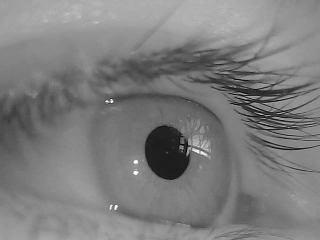
\includegraphics[width=.9\linewidth]{plots/orig_canny.png}
      \caption{Original frame}
      \label{fig:th_orig}
    \end{subfigure}%
    \begin{subfigure}{.5\textwidth}
      \centering
      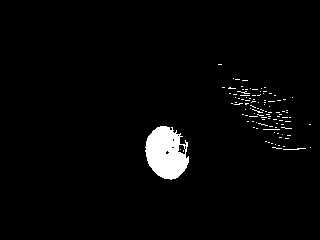
\includegraphics[width=.9\linewidth]{plots/thresholded.jpg}
      \caption{thresholded frame}
      \label{fig:th_thres}
    \end{subfigure}
    \caption{Original and thresholded frame}
    \label{fig:simple_thresh}
\end{figure}
In figure \ref{fig:simple_thresh}, it can be seen that the thresholding is extremely volatile to reflections, eyelashes and other noise, concluding that thresholding only has a good performance in a strictly defined environment with almost no noise. 

To showcase the volatility and dependency on the threshold value, figure \ref{fig:thresholded_images} shows a series of the same frame with different threshold values (Th). It can be seen that the threshold value has to be chosen very carefully. If the value is chosen too low, the pupil region is not found. If the value is chosen too high, too much information is extracted and the pupil region can not be differentiated from the rest. 


\begin{figure}[htbp]
    \centering
    \begin{tabular}{cccc}
    \begin{subfigure}{0.2\linewidth}
    \centering
    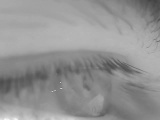
\includegraphics[width=\linewidth]{plots/thresholding/thresholded_eyelid.jpg}
    \caption{Original}
    \end{subfigure} &
    \begin{subfigure}{0.2\linewidth}
    \centering
    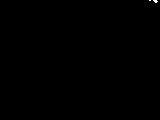
\includegraphics[width=\linewidth]{plots/thresholding/th1}
    \caption{Th = 65}
    \end{subfigure} &
    \begin{subfigure}{0.2\linewidth}
    \centering
    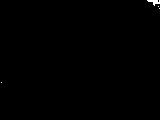
\includegraphics[width=\linewidth]{plots/thresholding/th2}
    \caption{Th = 71}
    \end{subfigure} &
    \begin{subfigure}{0.2\linewidth}
    \centering
    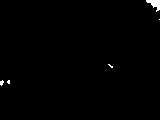
\includegraphics[width=\linewidth]{plots/thresholding/th3}
    \caption{Th = 77}
    \end{subfigure} \\
    \begin{subfigure}{0.2\linewidth}
    \centering
    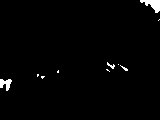
\includegraphics[width=\linewidth]{plots/thresholding/th4}
    \caption{Th = 83}
    \end{subfigure} &
    \begin{subfigure}{0.2\linewidth}
    \centering
    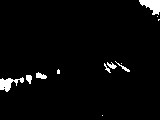
\includegraphics[width=\linewidth]{plots/thresholding/th5}
    \caption{Th = 89}
    \end{subfigure} &
    \begin{subfigure}{0.2\linewidth}
    \centering
    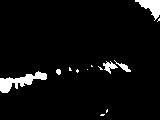
\includegraphics[width=\linewidth]{plots/thresholding/th6}
    \caption{Th = 95}
    \end{subfigure} &
    \begin{subfigure}{0.2\linewidth}
    \centering
    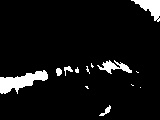
\includegraphics[width=\linewidth]{plots/thresholding/th7}
    \caption{Th = 101}
    \end{subfigure} \\
    \begin{subfigure}{0.2\linewidth}
    \centering
    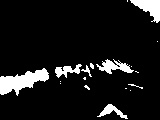
\includegraphics[width=\linewidth]{plots/thresholding/th8}
    \caption{Th = 107}
    \end{subfigure} &
    \begin{subfigure}{0.2\linewidth}
    \centering
    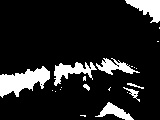
\includegraphics[width=\linewidth]{plots/thresholding/th9}
    \caption{Th = 113}
    \end{subfigure} &
    \begin{subfigure}{0.2\linewidth}
    \centering
    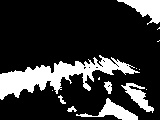
\includegraphics[width=\linewidth]{plots/thresholding/th10}
    \caption{Th = 119}
    \end{subfigure} &
    \begin{subfigure}{0.2\linewidth}
    \centering
    
\includegraphics[width=\linewidth]{plots/thresholding/th11}
    \caption{Th = 125}
    \end{subfigure} \\
    \begin{subfigure}{0.2\linewidth}
    \centering
    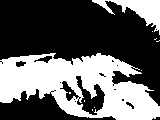
\includegraphics[width=\linewidth]{plots/thresholding/th12}
    \caption{Th = 131}
    \end{subfigure} &
    \begin{subfigure}{0.2\linewidth}
    \centering
    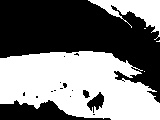
\includegraphics[width=\linewidth]{plots/thresholding/th13}
    \caption{Th = 137}
    \end{subfigure} &
    \begin{subfigure}{0.2\linewidth}
    \centering
    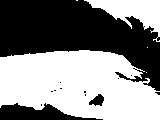
\includegraphics[width=\linewidth]{plots/thresholding/th14}
    \caption{Th = 143}
    \end{subfigure} &
    \begin{subfigure}{0.2\linewidth}
    \centering
    
\includegraphics[width=\linewidth]{plots/thresholding/th15}
    \caption{Th = 149}
    \end{subfigure} \\
    \end{tabular}
    \caption{Thresholded images}
    \label{fig:thresholded_images}
    \end{figure}

    \subsection{Ellipse fitting}
    \label{subsubsec:ellipsefitting}
    Ellipse fitting \cite{fitzgibbon_direct_2000} based on minimizing the algebraic distance using least squares fitting is a common method to fit an ellipse to a set of points. Given a set of $n$ 2D points $p_i = (x_i, y_i)$ where $i = 1,2,...,n$ and the equation of an ellipse in standard form is: 
    \begin{equation}
        F(x,y)=Ax2+Bxy+Cy2+Dx+Ey+F=0
        \label{eq:ellipse_standard}
    \end{equation}
    Where $a=[A, B, C, D, E, F]^T$ are the parameters to be determined. To exclude the trivial solution $a=0$, the constraint $||a||^2=1$ is added. Another important constraint is that the ellipse is not a hyperbola or a parabola. Therefore adding the constraint $B^2-4AC<0$ ensures ellipses as a result.
    Let's define the design Matrix $D$ as: 
    \begin{equation}
        D = \begin{pmatrix}
        x_1^2 & x_1y_1 & y_1^2 & x_1 & y_1 & 1 \\
        x_2^2 & x_2y_2 & y_2^2 & x_2 & y_2 & 1 \\
        \vdots & \vdots & \vdots & \vdots & \vdots & \vdots \\
        x_n^2 & x_ny_n & y_n^2 & x_n & y_n & 1 
        \end{pmatrix}
        \label{DesignMatrix}
        \end{equation}
    And let's define $C$ as the constraint matrix so that the constraint can be expressed as $a^TCa=1$

        \begin{equation}
            C = \begin{pmatrix}
            0 & 0 & 2 & 0 & 0 & 0 \\
            0 & -1 & 0 & 0 & 0 & 0 \\
            2 & 0 & 0 & 0 & 0 & 0 \\
            0 & 0 & 0 & 0 & 0 & 0 \\
            0 & 0 & 0 & 0 & 0 & 0 \\
            0 & 0 & 0 & 0 & 0 & 0 \\
            \end{pmatrix} \label{eq:C}
        \end{equation}
Now the method of Lagrange multipliers \cite{gander_least_1980} gives the conditions for solving the least square fit with the scatter matrix being $S=D^TD$: 
\begin{gather}
    Sa = \lambda Ca \\
    a^TCa=1
\end{gather}
This return at most six solutions for $a_j$ and $\lambda_j$. The solution with the smallest $\lambda_k$ and the corresponding eigenvector $a_k$ best fits the ellipse based on the least square fit. 
\subsection{Contours}
When working with thresholds, the contour is of interest. The contour is defined as the outer boundary of the threshold binary matrix and is the foundation for the ellipse fit method. 
Here it is not given to extract only one contour from the binary mask; therefore, the contours need to be filtered based on which contour represents the pupil the best. 
Mainly three criteria are used. 

\subsubsection{Circularity / Compactness}
Circularity is described  as the contour area $\mathsf{A} $ multiplied with $4\pi$ and divided by the integral over the outer boundary of the contour, also known as the permitter of the contour.
\begin{equation}
    \text{circularity} = \frac{4\pi\mathsf{A} }{(\oint_{\partial S} dS)^2}
\end{equation}

\subsubsection{Similarity }
For calculating similarity, the OpenCV library is used. This method compares a given shape with another. As the base for the comparison, a simple ellipse is taken and then compared with all possible contours.

\subsubsection{Area}
The Area of the contour should be maximal to find the largest pupil area and filter out smaller area contours. 
Each algorithm that returns a list of contours needs to be checked with these three conditions, and in the best-case scenario, only the pupil's contour survives. The result is then the contour on which an ellipse can be fitted. 
\newpage
\section{Random Sample Consensus (RANSAC) }
\label{sus:ransac}
The Random Sample Consensus (RANSAC) \cite{derpanis_overview_2010} algorithm is an iterative method used to estimate the parameters for a known problem. For ellipse fitting, a contour or a set of possible points inside or on the contour $C$ is the input. The algorithm then randomly selects a subset $S_c$ of 5 randomly selected points in $C$. 
These 5 points are then used to fit an ellipse as described in the section Ellipse Fitting.

\begin{figure}[h]
    \centering
    \begin{tikzpicture}[scale=0.4]
        % Drawing the coordinate system
        \draw[->] (-1,0) -- (12,0) node[right] {$x$}; % x-axis
        \draw[->] (0,-1) -- (0,12) node[above] {$y$}; % y-axis
        
        % Drawing the ellipse
        \draw[rotate around={30:(8,8)},scale=1] (8,8) ellipse (7cm and 5cm);
        
        % Annotations
        \node at (8,7) {$(h,k)$};
        \draw [rotate around={30:(8,8)},scale=1] (8,8) -- ++(7,0) node[midway,above] {$a$};
        \draw [rotate around={30:(8,8)},scale=1] (8,8) -- ++(0,5) node[midway,right] {$b$};
        \draw[scale=1, red] (8,8) -- ++(4.5,0) node[midway,above] {$\theta$};
        \draw[scale=1, red] (8,8) ++(4,0) arc (0:30:4);
        \filldraw[black] (8,8) circle (2pt);

    \end{tikzpicture}
    \caption{Ellipse with center $(h,k)$, semi-axes $a$ and $b$, and rotation $\theta$}
    \label{fig:sampleellipse}
\end{figure}
The equation \ref{eq:ellipsequation} represents an ellipse with major axis $a$, minor axis $b$, and the ellipse's center at $(h,k)$. The angle $\theta$ is the ellipse rotation in the coordinate system.
\begin{equation}
    \frac{((x-h)\cos(\theta) + (y-k)\sin(\theta))^2}{a^2} + \frac{((x-h)\sin(\theta) - (y-k)\cos(\theta))^2}{b^2} = 1
    \label{eq:ellipsequation}
\end{equation}

When comparing the ellipse equation \ref{eq:ellipsequation} with the general covariance ellipse equation \ref{ellipseco}
\begin{equation}
    \mathbf{A}x^2 + \mathbf{B}xy + \mathbf{C}y^2 = 1
    \label{ellipseco}
\end{equation} 
and compare coefficients, a relation between the ellipse parameters and the covariance matrix can be found
\begin{align}
    \mathbf{A}&=a^2 * \sin (\theta)^2 + b^2*\cos (\theta)^2 \\
    \mathbf{B}&= 2(a^2-b^2)*\sin (\theta)*\cos (\theta) \\
    \mathbf{C}&= a^2*\cos (\theta)^2 + b^2*\sin (\theta)^2
    \label{coefficients}
\end{align}

The covariance matrix is :
\begin{equation}
    \mathbf{V} = \begin{bmatrix}
        \mathbf{A} & \mathbf{B} \\
        \mathbf{B} & \mathbf{C} 
    \label{covariance}
    \end{bmatrix}
\end{equation}
The benefit of using the covariance matrix is that the eigenvalues and eigenvectors directly relate to the major and minor axis and the rotation of the ellipse. The eigenvalues represent the axis's major and minor, and the eigenvectors represent the rotation matrix $R$ that rotates the ellipse in the coordinate system. 

Important to note is that the eigenvectors need to be ordered to the size of the eigenvalues, and the eigenvector calculated with the largest eigenvalue comes first. This has the benefit that all parameters are known to transform all points into a new coordinate system where the calculated ellipse equation is represented in a unit circle.


\begin{figure}[h]
    \centering
    \begin{tikzpicture}
        % Draw the circle with radius 1
        \draw (0,0) circle (1);
        
        % Draw the axes
        \draw[->] (-1.5,0) -- (1.5,0) node[right] {$x$};
        \draw[->] (0,-1.5) -- (0,1.5) node[above] {$y$};
        
        % Define the angle
        \def\angle{30}
        
        % Draw the angle arc
        \draw (1,0) arc (0:\angle:1);
        
        % Draw the line and label
        \draw[->,red] (0,0) -- (\angle:1) node[right] {$r=1$};
        
        % Draw the labels for the trigonometric identities
        \node at (1.3,-1) {$\cos \theta = x$};
        \node at (-1,1.3) {$\sin \theta = y$};

    \end{tikzpicture}
    \caption{Unit circle with trigonometric identities}
    \label{fig:unit_circle}
\end{figure}

Using the unit circle allows for a simple distance calculation. Because $\lambda_{1,2}$ are known, then all points in $\in C$ of the old coordination system can be transformed onto the unit circle by subtracting $x-h$ and $y-k$, are then multiplied by the transposed eigenvectors to rotate the points into the new system and then divide by the eigenvalues. Let $p$ be a point in $C$ and $p'$ the transformed point in the new coordinate system. 
\begin{align}
    p' = R^T \begin{bmatrix} p_x - h \\ p_y - k \end{bmatrix} \odot \begin{bmatrix} \frac{1}{\lambda_1} \\ \frac{1}{\lambda_2} \end{bmatrix}\\
    r = \sqrt{p_x'^2 + p_y'^2}
    \label{distance calculation}
\end{align}
So the distance calculation of a point $p$ to the ellipse curve simplifies to the distance of the transformed point $p'$ to the unit circle.
\begin{equation}
    d = \sqrt{p_x'^2 + p_y'^2} -1
\end{equation}

The RANSAC algorithm iterates $n$ times to find the best ellipse with the most inliers. The points are classified into three groups: 
\begin{equation}
    p =\begin{cases}
    \text{inlier} = \{p \in C | d < 0\}\\
    \text{border} = \{p \in C | d = 0\}\\
    \text{outlier} = \{p \in C | d > 0\}
    \end{cases}
    \label{inliers}
\end{equation}
The RANSAC algorithm calculates the ellipse parameters with five random points $S_c$ for $n$ iterations and evaluates the number of inliers for each iteration. The ellipse with the most inliers is considered the best fit. 

The differentiation between on-border and inlier is essential to weigh the focus on enclosing ellipses. Because the distance calculation does not return an integer, it is possible that the distance is not exactly zero, but the point $p$ is on the border. So it is crucial when comparing floats with each other to always use a small epsilon value that $d$ can differ from 0. This epsilon is also defined as threshold. 
In Python, functions like \textit{isclose} can be used to compare floats with each other. The number of iterations to get a 99\% chance of finding the best ellipse with the most inliers can be calculated with the following formula: 
\begin{equation}
    n = \frac{\log(1-P)}{\log(1-w^s)}
    \label{iterations}
\end{equation}
Where $P$ = is the probability of finding the best ellipse and $w$ is the ratio of inliers to outliers (Probability that a point is an inlier). This formula estimates the number of iterations $n$ for the RANSAC algorithm to be 99\% sure to find the best ellipse with $s$ samples taken each iteration. 

In ellipse fitting $s=5$, $p=0.99$, and for $w$, an approximation must be made. Because the number of inliers is unknown, the ratio of inliers to outliers can not be calculated and needs to be estimated. In this case, we assume that the ratio of inliers to outliers is $w=0.90$ which can be adapted later on. 
\begin{equation}
    n = \frac{\log(1-0.99)}{\log(1-0.90^5)} =  5.158
\end{equation}
So the number of iterations to find the best ellipse with the most inliers is 6. But it is important to keep in mind that this is only true if 90\% of the points are located on the ellipse contour. Otherwise, the number of iterations needs to increase because the ratio of inliers to outliers changes drastically. Also an important fact is that the number of iterations needs to be chosen high enough because throughout the video, the number of border points changes drastically, and $n$ can not be estimated perfectly. Therefore $n$ is set to $500$ but can still be optimized.

If only the border points are considered inliers and only $\frac{1}{5}$ of the border is visible, the number of iterations would jump to $4'713$. The calculation of the inliers is discussed in detail in section: \ref{sus:acwe_ransac}.
\newpage
Visualizing RANSAC looks like this:
\begin{figure}[h]
    \centering
    \begin{subfigure}{0.3\textwidth}
        \centering
        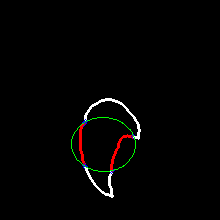
\includegraphics[width=0.9\linewidth]{plots/ransac/test_mask98.png}

    \end{subfigure}%
    \hfill
    \begin{subfigure}{0.3\textwidth}
        \centering
        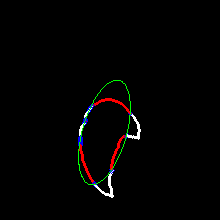
\includegraphics[width=0.9\linewidth]{plots/ransac/test_mask186.png}

    \end{subfigure}%
    \hfill
    \begin{subfigure}{0.3\textwidth}
        \centering
        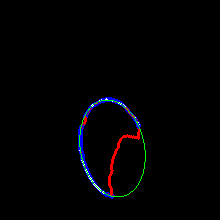
\includegraphics[width=0.9\linewidth]{plots/ransac/test_mask112.png}

    \end{subfigure}%
    \caption{Example of RANSAC ellipse fit iterations}
    \label{fig:RANSAC_it}
\end{figure}

In figure \ref{fig:RANSAC_it}, the green ellipse is the ellipse fitted to the five randomly chosen points. The red points are the inliers of the ellipse, and the blue points are the points that lay on the boundary within a given threshold. The white points are the outliers of the ellipse. The number of inliers is the sum of the red points and the number of boundary points is the sum of blue points. The goal is to find the ellipse with the most inliers, boundary points, and smallest area. These conditions lead to an enclosing ellipse with minimal area. All points together are the contour of the binary mask received from the ACWE algorithm explained in section \ref{sus:acwe}.
\newpage
\section{Active Contouring }
Active contour segmentation \cite{vondracek_image_2018} is a method that is used to find the boundary curve of an object given that the object exists. There are many different approaches in active contouring, but three variants will be discussed in this thesis. The first one is the classic Snakes approach (Kass et al., 1988) \cite{kass_snakes_1988} with a simple energy function, and the second variant is the active contouring without edges (ACWE)  based on level sets. The third variant is active contouring with ellipse parameters. In all cases, an initial contour is set, and through iterative changes, tries to find the boundary curve of an object. In each iteration the contour is changed by a small amount and then evaluated with an energy function. The energy function is a measurement of how well the contour fits the contour of the object, and in both cases, the energy function is minimized.

Let $C(q): [0, 1] \rightarrow \mathbb{R}^2$ be a parametrized planar curve and let $I : [0, a] \times [0, b] \rightarrow \mathbb{R}^+$ be a given image used to detect the object boundaries with active contouring. The classical snake's approach (Kass et al., 1988) \cite{kass_snakes_1988} associates the curve $C$ with an energy given in \refeq{acgd}
But the most basic description for the energy minimization can be summarized in $E_{int}$ and $E_{ext}$. 
\begin{equation}
    E = E_{int} + E_{ext}
    \label{energy}
\end{equation}
\begin{equation}
        E(C) = \underbrace{\alpha \int_0^1 |C'(q)|^2 \, dq + \beta \int_0^1 |C''(q)|^2 \, dq}_{\text{E}_{int}} - \underbrace{\lambda \int_0^1 |\nabla I (C(q))| \, dq}_{\text{E}_{\text{ext}}}
\label{acgd}
\end{equation}
The goal is to minimize the energy function, and by doing so, the contour $C$ will find local minima and depending on the sign of $\lambda$ be attracted to light or dark edges. The first two terms of the energy describe the internal energy of the contour and the last term represents the external energy. In other words, the internal energy describes the curve's smoothness and the external energy describes the relation of the curve to the edge at the curve's boundary. In the following, the these terms will be discussed in more detail.

To use these Equations, they have to be applied on a discrete grid. The curve $C$ is discretized into $N$ points  $c_i(x_i,y_i)$ with $i \in [0, N-1]$. The energy function is then calculated for each point $c_i$ and summed up to get the total energy of the curve. The energy function is minimized by using the gradient descent method. The gradient of the energy function is calculated and the points $c_i(x_i,y_i)$ are changed by a small amount in the direction of the gradient. The gradient descent method is repeated until the energy function converges to a local minimum or the optimal solution. 

The formula can be discretized by sampling the initial curve position evenly, then the formula can be expressed as: 

\begin{equation}
    E = \sum_{i=0}^{N-1} \alpha (c_{i+1} - c_i)^2 + \beta (c_{i+2} - 2c_{i+1} + c_i)^2 - \lambda |\nabla I (c_i)|
\end{equation}
Here it is important to note that the points are circular, when $i$ equals $N-1$, the next point is $c_0$. Therefore the indices can also be interpreted as $c_{(i+1 \bmod N)}$ and $c_{(i+2 \bmod N)}$
\begin{align*}
    \text {substitute:} \begin{cases}
    \sum_{i=0}^{N-1}(c_{i+1} - c_i) = C'(q) \\
    \sum_{i=0}^{N-1}(c_{i+2} - 2c_{i+1} + c_i) = C''(q)
    \end{cases}
\end{align*}

Where $C'(q)$ calculates the length of the curve and $C''(q)$ calculates the curve's curvature.  

Because the classic Snakes implementation searches for the best boundary curve that locally minimizes the energy function, the contour must be initialized close to the best solution. Otherwise, the algorithm will converge to a local minimum and not the global minimum. The classic Snakes approach searches for the minima with PDEs that are solved using the steepest descent method, which brings performance issues and is prone to terminate early if a local minimum is found. 

\subsection{Active Contouring without Edges (ACWE) }
\label{sus:acwe}
In ACWE \cite{vondracek_image_2018}, the same principle is used to find the best object boundary. But in this case, the energy function is minimized using level sets and morphological operations to solve the PDEs. The morphological operations use four different structuring elements. 

\begin{figure}[ht]
    \centering
    \begin{subfigure}[b]{0.23\textwidth}
        \centering
        \begin{tikzpicture}[scale=0.6]
            \draw (0,0) grid (3,3);
            \filldraw[fill=black!80] (0,3) rectangle (1,2);
            \filldraw[fill=black!80] (2,0) rectangle (3,1);
            \filldraw[fill=black!80] (1,1) rectangle (2,2);
        \end{tikzpicture}
        \caption{Element 1}
        \label{fig:e1}
    \end{subfigure}%
    \begin{subfigure}[b]{0.23\textwidth}
        \centering
        \begin{tikzpicture}[scale=0.6]
            \draw (0,0) grid (3,3);
            \filldraw[fill=black!75] (1,0) rectangle (2,1);
            \filldraw[fill=black!75] (1,2) rectangle (2,3);
            \filldraw[fill=black!75] (1,1) rectangle (2,2);
        \end{tikzpicture}
        \caption{Element 2}
        \label{fig:e2}
    \end{subfigure}
    \begin{subfigure}[b]{0.23\textwidth}
        \centering
        \begin{tikzpicture}[scale=0.6]
            \draw (0,0) grid (3,3);
            \filldraw[fill=black!75] (0,0) rectangle (1,1);
            \filldraw[fill=black!75] (2,2) rectangle (3,3);
            \filldraw[fill=black!75] (1,1) rectangle (2,2);
        \end{tikzpicture}
        \caption{Element 3}
        \label{fig:e3}
    \end{subfigure}%
    \begin{subfigure}[b]{0.23\textwidth}
        \centering
        \begin{tikzpicture}[scale=0.6]
            \draw (0,0) grid (3,3);
            \filldraw[fill=black!75] (0,1) rectangle (1,2);
            \filldraw[fill=black!75] (2,1) rectangle (3,2);
            \filldraw[fill=black!75] (1,1) rectangle (2,2);
        \end{tikzpicture}
        \caption{Element 4}
        \label{fig:e4}
    \end{subfigure}%

    \caption{The four morphological structuring elements used in ACWE.}
    \label{fig:neighborsmorph}
\end{figure}
ACWE is based on Geodesic Active Contours (GAC) \cite{vondracek_image_2018}. GAC can already solve critical problems from classical active contouring. Based on a threshold, the contour is iteratively evaluated and then compared to the threshold to decide if it flows and expands the contour to a new pixel. GAC is based on classic active contours and geodesic curves in a Riemannian space. The level sets have the benefit that they can easily be implemented in a discrete grid and open the door to solve the PDEs using morphological operations. The level set approach brings more stability and is less sensitive to the initial contour than the classical active contouring method. It is also possible to detect the interior and exterior boundary of an object. In the classical approach, the internal force is based on the first and second derivatives of the curve and results in stability, computational complexity, and performance issues. The internal energy is solved in the GAC by using the evolution of an implicitly defined curve. The GAC algorithm is based on a level set function $u$ and is defined as:
\begin{equation}
    \frac{\partial u}{\partial t} = 
    \underbrace{g(I) \cdot |\nabla u| \cdot \text{div} \left(\frac{\nabla u}{|\nabla u|}\right)}_{\text{Smoothing force}} 
    + \underbrace{g(I) \cdot \nu \cdot |\nabla u|}_{\text{Balloon force}} 
    + \underbrace{\nabla g(I) \cdot \nabla u}_{\text{External force}}.
    \label{deform}
    \end{equation}
    
Where $u$ is the level set function described as a binary mask. $u$ is 1 inside the mask and 0 outside. $I$ is the image and $g(I)$ is the edge indicator function. $\nu$ is a variable that decides in which direction and how strong the curve should move. 
For choosing $g(I)$, there are different variants but two of the most common are the following: 

\begin{equation}
    g(I) = \begin{cases}
     1/(1 + |\nabla I|*\alpha) &(1)\\
     -|\nabla I| &(2)
    \end{cases}
\end{equation}
In (1) $g(I)$ is low when the gradient is high and vice versa. Meaning that $g(I)$ regulates the influence of the forces depending on the gradient. It is around 0 when the gradient is high. In other words, the curve stops moving when the pixel has reached an intensity transition, such as an edge. $\alpha$ is a variable that regulates how strong the influence of the external energy is. In (2) $g(I)$ is negative when the gradient is high. So both definitions of $g(I)$ will stop the curve from moving when it reaches an edge.

\subsubsection{Smoothing Force}
The smoothing force is the approximation of the curvature term of the classical snake's method. The difference is that in GAC, the smoothing force is calculated using the gradient of the level set function $u$ instead of the curve. 
\begin{equation}
    g(I) \cdot |\nabla u| \cdot \text{div} \left(\frac{\nabla u}{|\nabla u|}\right)
\end{equation}
The smoothing force is calculated using a recursive call of $SI$ and $IS$. Together they build operator $F(u)$, which approximates the curvature flow based on PDEs. 
\begin{equation}
    \text{F}(u) = SI(u)\circ IS (u)
    \label{eq:smoothingforce}
\end{equation}
Where SI means supremum of infimum and IS means infimum of supremum. In other words, SI stands for eroding the current level set $u$ four times separately with each of the structuring elements once and taking for each pixel its highest result, and IS stands for dilating the current level set $u$ four times separately with each of the structuring elements once and taking for each pixel its lowest result. One step of smoothing looks like the following: 
\begin{align*}
    1) u_{SI\circ IS}=\text{erode}(u) \circ \text{dilate}(u) \\
    2) u_{IS\circ SI}=\text{dilate}(u) \circ \text{erode}(u)
\end{align*}
by repeating step 1 and step 2 the smoothing force can be stronger or weaker. But it is crucial to always use step 1 and step 2 in the same order. 


\subsubsection{Balloon Force}
The balloon force is essential in regions where the gradient is low and hinders the curve flow from getting stuck at a local minimum. Especially when looking at the external force, where the velocity of the curve is determined by the gradient of $g(I)$ and the gradient of $u$. If $g(I)$ goes to zero, the curve will have no external velocity. Therefore the balloon force is vital to make the algorithm more robust.
\begin{equation}
    g(I) \cdot \nu \cdot |\nabla u|
\end{equation}
In GAC, the ballon is also calculated differently than in the classical snake's method. 
The Balloon force $g(I)*|\nabla u| *v$ with parameter $v \in  {-1,1}$ can be substituted with dilation using the four different neighborhood structuring elements and then taking for every pixel the minimum value received from the four dilations. Dilation is a morphological operation and is computed very efficiently and also gets rid of the PDEs that are solved in the classical snake's method. By using dilate, the balloon force leads to the desired result of making the curve grow. 
\begin{equation}
    \text{dialate}(u)  =  u \bigoplus Element_i \quad \text{for} \quad i \in \{1,2,3,4\}
    \label{dialate}
\end{equation}

\subsubsection{External force}
The external force is the same as in the classical snake's method, but in GAC, it is weighted by $g(I)$ to stop the curve from moving when it reaches an edge.
\begin{equation}
    \nabla g(I) \cdot \nabla u
\end{equation}
The change in the level set function $u$ is only applied to the points where $g(I) > T$, where $T$ is a defined threshold to control the velocity and leads to the characteristic that the curve moves faster in areas where the gradient is low. In other words, it leads to an algorithm that moves faster in a region with the same intensity and slower in regions with a high gradient. 

The external force or the attracting force is calculated for each point $p$ in the binary mask from the before modified level set function $u$ and evaluated with the following equation:
\begin{equation}
    p = \begin{cases}
        1 &iff  \nabla u * \nabla g(I) > 0 \\
        0 &iff \nabla u * \nabla g(I) < 0
    \end{cases}
    \label{eq:externalforce}
\end{equation}
\subsubsection{Summary}
To conclude, the equation \refeq{eq:externalforce} describes the deformation of $u$, the binary level set function. and is the main equation for Geodesic Active Contours (GAC). 

\subsection{Convert GAC to ACWE}
\label{sus:GACtoACWE}
The GAC only iteratively inspects places where the curve could move, and there lies the main difference to the ACWE. ACWE, also known as the Chan-Vese algorithm, considers the complete image to evaluate the boundary or curvature flow of the level set. 
Let $c_i$ be the mean intensity of a subset $\Omega$ of the image $I(x,y)$. Let $c_1$ be the mean intensity inside the curve or level set $u$ defined as $\Omega_1$ and $c_2$ the mean intensity outside the level set $u$ defined as $\Omega_2$. 
\begin{equation}
    c_{i}= \frac{ \int_{\Omega_{i}} I(x) \,dx}{\int_{\Omega_{i}} \, dx }
    \label{eq:meanintensity}
\end{equation}
Then the external force function $F(c_1,c_2,C)$ is defined as
\begin{equation}
    \begin{split}
    F(c_1, c_2, C) = & \mu \cdot \text{length}(u) + \nu \cdot |\text{inside}(u)| \\
    & + \lambda_1 \cdot \int_{\Omega_1} (I(x) - c_1)^2 \, dx \\
    & + \lambda_2 \cdot \int_{\Omega_2} (I(x) - c_2)^2 \, dx
    \end{split}
    \label{eq:curvatureflow}
    \end{equation}

where the first two terms $\mu \cdot \text{length}(u) + \nu \cdot |\text{inside}(u)|$ are the same as in the GAC. The third and fourth terms calculate the unscaled intensity variance in the different subsets $\Omega_1$ and $\Omega_2$. 

The only difference between GAC and ACWE is that the external force is calculated differently. In GAC, the external force is evaluated with $\nabla g(I) \cdot \nabla u$ and then, based on a threshold, decides if a point is inside or outside the curve, as seen in equation \refeq{eq:externalforce}. 

In ACWE, the external force is calculated with the mean intensity of the subsets $\Omega_1$ and $\Omega_2$ and the intensity of the image $I(x)$ as seen in equation \refeq{eq:curvatureflow}. Converting the equation onto a discrete grid it can be written as: 
\begin{equation}
   \xi  = \underbrace{\lambda_{1} \cdot | \nabla u_{mask}| \cdot (I(x)-c_{1})^{2}}_{Inside}-\underbrace{\lambda_{2} \cdot|\nabla u_{mask}| \cdot (I(x)-c_{2})^{2}}_{outside}
\end{equation} 
$\xi$ is then used to evaluate the new points in the level set function $u$ with the following condiction:
\begin{equation}
    u(x,y) = \begin{cases}
        1 \text{ if } \xi<0 \\
        0 \text{ if } \xi>0 \\
        \text{do nothing otherwise}
        \end{cases}
\end{equation}
The gradient of the mask will only be nonzero at the contour of the mask. 
Now the mean is subtracted from $I(x)$, and each point on the contour will have two values, their inside and outside weighted intensities. By subtracting the mean intensity from the pixel intensities on the boundary of u, multiplying it with $\lambda_i$ and subtracting the outside term from the inside term, a relationship between the inside and outside intensities is created and can be tuned with the sensitivity parameters $\lambda_i$ . 

This relationship is then used to calculate the new points in the level set function $u$ and the process is repeated until the level set function converges. When the level set reaches the object boundary, the inside and outside intensities will be the same, the curve will not move anymore, and the equation will go to zero. 
Here is an example of the evolution the level set $u$ when the ACWE algorithm is used with a given starting point inside the pupil. 
\begin{figure}[h]
    \centering
    \begin{subfigure}{0.3\textwidth}
        \centering
        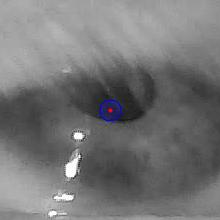
\includegraphics[width=0.9\linewidth]{plots/acwe/iteration_0.png}
        \caption{Initial level set}
    \end{subfigure}%
    \hfill
    \begin{subfigure}{0.3\textwidth}
        \centering
        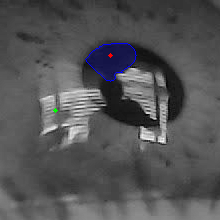
\includegraphics[width=0.9\linewidth]{plots/acwe/iteration_15.png}
        \caption{Iteration 15}
    \end{subfigure}%
    \hfill
    \begin{subfigure}{0.3\textwidth}
        \centering
        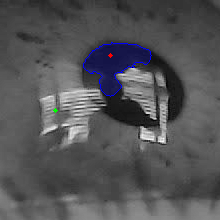
\includegraphics[width=0.9\linewidth]{plots/acwe/iteration_30.png}
        \caption{Iteration 30}
    \end{subfigure}%
    \hfill
    \begin{subfigure}{0.3\textwidth}
        \centering
        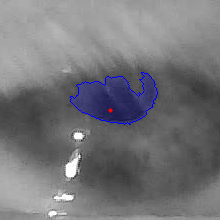
\includegraphics[width=0.9\linewidth]{plots/acwe/iteration_60.png}
        \caption{Iteration 60}
    \end{subfigure}
    \hfill
    \begin{subfigure}{0.3\textwidth}
        \centering
        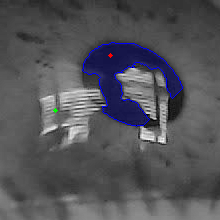
\includegraphics[width=0.9\linewidth]{plots/acwe/iteration_90.png}
        \caption{Iteration 90}
    \end{subfigure}
    \hfill
    \begin{subfigure}{0.3\textwidth}
        \centering
        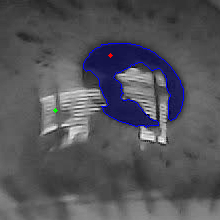
\includegraphics[width=0.9\linewidth]{plots/acwe/iteration_115.png}
        \caption{Iteration 115}
    \end{subfigure}
    \caption{ACWE iterations}
    \label{fig:iterations_acwe}
\end{figure}

\newpage
\subsection{Active contouring with ellipse parameters}
A different approach is to let an ellipse grow and modify its parameters based on the gradient information. By sampling an amount of equally spaced points on the ellipse and evaluating an energy function based on the scalar product of the image intensity gradient vector  and the normal vector of the ellipse at those points. 
\begin{equation}
    E = -\sum_{i=0}^{N-1} \nabla I(p_i) \cdot \vec{n(p_i)}
\end{equation} 
Where $p_i$ is a point on the ellipse and $\vec{n(p_i)}$ is the normal vector of the ellipse at that point. $\nabla I(p_i)$ is the gradient of the image at point $p_i$. The energy function is iteratively minimized by changing the ellipse parameters.
\begin{figure}[h]
    \centering
    \begin{tikzpicture}[scale=0.6, transform shape]
        \def\a{3} % semi-major axis
        \def\b{2} % semi-minor axis
        \def\scale{1} % scale for normal and gradient vectors
    
        % Draw ellipse
        \draw (0,0) ellipse (\a cm and \b cm );
        
        % Draw 10 points and corresponding vectors
        \foreach \i in {1,2,...,10} {
            \pgfmathsetmacro{\angle}{\i*36}
            \pgfmathsetmacro{\xcoord}{\a*cos(\angle)}
            \pgfmathsetmacro{\ycoord}{\b*sin(\angle)}
            \coordinate (p\i) at (\xcoord,\ycoord);
            \fill (p\i) circle (1.5pt);
    
            % Normal vector
            \draw[->, blue, thick] (p\i) -- ++({\xcoord/\a^2*1.5*\scale},{\ycoord/\b^2*1.5*\scale});
    
            % Dummy gradient vector
            \draw[->, red, thick] (p\i) -- ++({\scale*cos(\angle+\i*0.5)},{\scale*sin(\angle+45+\i*0.5)});
        }
    \end{tikzpicture}
    \label{fig:normalgradientellipse}
    \caption{Ellipse with normal vector (blue) and gradient vectors (red)}
    
    \end{figure}
Finding the best fit turns into a minimization problem. The energy function still needs a term to ensure the curve grows and does not get stuck at a local minimum. Here it is not possible to use the morphological operators because the shape of the ellipse is not given as a level set. Instead the ellipse is based on only the five ellipse parameters: center$(x,y)$, axis: $(a,b)$, angle $\theta$. 

The energy function is the lowest when at each point, the gradient vector and normal vector have the same direction, and the magnitude of the gradient is maximal. The gradient vector consists of the magnitude of the gradient and the orientation. Whereas the normal vector is normalized and points outwards in the direction of the normal of the ellipse curve at that point. 

The problem with this approach is overlapping with classical active contouring. The initial contour needs to be close to the optimal solution. Otherwise, the algorithm stops at a local minimum, and convergence to the optimal solution is not guaranteed. Because it is a minimization with five parameters, it is a very complex problem, and the algorithm needs multiple iterations to find the best local solution. 

For this approach, the image needs preprocessing and the algorithm is very sensitive to noise. Therefore, first applying a low pass filter onto the image is a must. But because of blurring, the image gradients and directions are not as accurate as they could be and the scalar product struggles with reflections and other noise.

Here is an example with the convergence to a local minimum. The initial ellipse was initialized far from the optimal solution and the algorithm converges to a local minimum. 

\begin{figure}[h]
    \centering
    \begin{tabular}{cc}
        \centering
        \begin{subfigure}{0.3\textwidth}
            \centering
            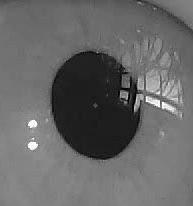
\includegraphics[width=0.9\linewidth]{plots/eye_dataset/roi.png}
            \caption{ROI}
        \end{subfigure} &
        \begin{subfigure}{0.3\textwidth}
            \centering
            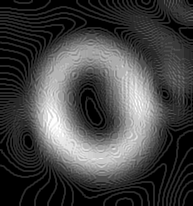
\includegraphics[width=0.9\linewidth]{plots/eye_dataset/mag.png}
            \caption{Gradient Magnitude}
        \end{subfigure} \\
        \begin{subfigure}{0.3\textwidth}
            \centering
            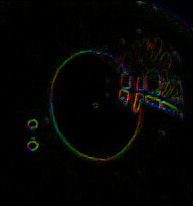
\includegraphics[width=0.9\linewidth]{plots/eye_dataset/direction.png}
            \caption{Gradient Direction}
        \end{subfigure}   &
        \begin{subfigure}{0.3\textwidth}
            \centering
            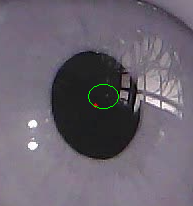
\includegraphics[width=0.9\linewidth]{plots/eye_dataset/result.png}
            \caption{Result}
        \end{subfigure}

    \end{tabular}
    \caption{Convergence to local minimum}
    \label{fig:ac_ellipse_gradient}
    \end{figure}

The problem with expanding the energy function with more terms is that the algorithm gets more complex. For example, when the size of the ellipse is used as a reward for the energy function (the bigger, the better), it is not given anymore that the minimization stops at the object's boundary. The parameters must be chosen carefully to ensure the algorithm converges to the optimal solution. 


\chapter{Algorithm Implementation}
In this chapter some of the algorithm in the theory chapter are combined, tested and evaluated. The goal is to find the most robust combination of algorithms to detect the pupil even in a very demanding data set like the LPW. The LPW data set is already discussed in its chapter and will not be discussed here again. In general the evaluation can be split up into two part. The first part is localization of the pupil and second part is finding the pupil ellipse. The importance of the localization is that with the information of the location of the pupil it is possible to create a region of interest (ROI). This has the benefit that in the second part the image size is already decreased and additional noise can be even more limited. Also the computational effort is reduced because the image size is smaller. Important to note is, that all algorithms make the basic assumption, that the pupil is always visible. So blinking is not counted as a failure and excluded of the evaluation if possible. For detecting blinking, other algorithms need to be used to preprocess every frame and detect if the eye is closed or not. 


\section{Localization}
For the localization mainly thresholding, edge detection and haar-like features were implemented and can now be evaluated. To make thresholding more flexible a semi adaptive algorithm was created to choose the best fitting threshold value. The histogram is used to determine the highest peak in the low intensity range. This value is then used to threshold the image. 
\begin{equation}
    t = \text{argmax} \{h(i) | i \in [0,255]\}
\end{equation}
With $h(i)$ being the histogram of the image. The threshold value is then used to calculate a range for using double thresholding to extract the pupil. The image is modified by setting all values below and above the threshold value to 0. 
\begin{equation}
    f(x,y)= \begin{cases}
        0 &iff \quad I(x,y) < t-35 \quad \text{or} \quad I(x,y) > t+25 \\
        I(x,y) &otherwise
    \end{cases}
\end{equation}
\subsection{Thresholding}
Whereas the under limit of the threshold is set lower than the higher limit. This derives from testing and can be concluded, that the probability that the pixels with lower intensity values belongs to the pupil is higher than the probability that the pixels with higher intensity values belong to the pupil. In a environment with almost no noise and most important no reflections this approach works very well. But as also already mentioned in the theory section, reflections lead to a less higher peak in the histogram and the possibility exist that the threshold value has no peak in the lower values range and therefore leads to a faulty result that can not be used to create an ROI or use it with edge detection to find the boundary of the pupil. Also it is important to note that with this thresholding approach the mask created is not a binary mask but a mask with values between $[t-35, t+25]$. But the possibility to use the binary mask still exist and the all contours found in this threshold range are evaluated by their circularity and similarity to an ellipse. The best fitting contour is then used to create the ROI or ellipse fit directly to find the ellipse parameters. 
[RESULTS]
This method works in a environment with almost no noise flawless, it is has benefit to reach the goal in almost realtime but in with the LPW data set it is keen to strugle with most of the conditions and is therefore not usefull for the LPW data set.

\subsection{Edge detection}
Edge detection is strongly effected by noise and therefore the preprocessing is key for useful results. Every frame undergoes the same preprocessing as in the other algorithms but a gaussian blur is used additionally to smooth fast changing intensity regions out.  Even though the gaussian blur is used, there is still information missing that is covered by noise. The edges are detected but the same problem as with thresholding arises here. By using Sobel and than the Canny edge detection the results are useful in a environment with almost no noise but as already said, LPW is known for its noise and reflections. Canny edge detection needs two threshold parameters to work properly and also here arises the problem that these parameters need to be adaptive to the environment which can be tricky. 
[RESULTS]

\subsection{Haar-like features}
The Haar-like feature is the approach that is proposed by this thesis to find the region of interest. It has the best detection rate of all approaches tested on the LPW data set and is therefore the best approach to find the ROI. The Haar-like feature is constructed as described in the theory part and is shown in \ref{fig:haar_pupil}. 
The calculation of the feature vector is done by using the integral image and is done 3 times with variating Radius $r$ all feature vectors are then compared and the location of the highest response is returned as a point that lies on the pupil. 

\begin{figure}[h]
    \centering
    \begin{subfigure}{0.5\textwidth}
        \centering
        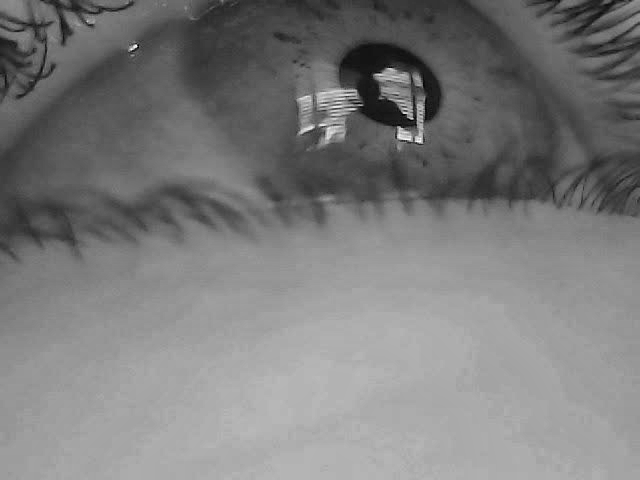
\includegraphics[width=0.9\linewidth]{plots/results/originalbest.png}
        \caption{Original Frame}
    \end{subfigure}%
    \hfill
    \begin{subfigure}{0.5\textwidth}
        \centering
        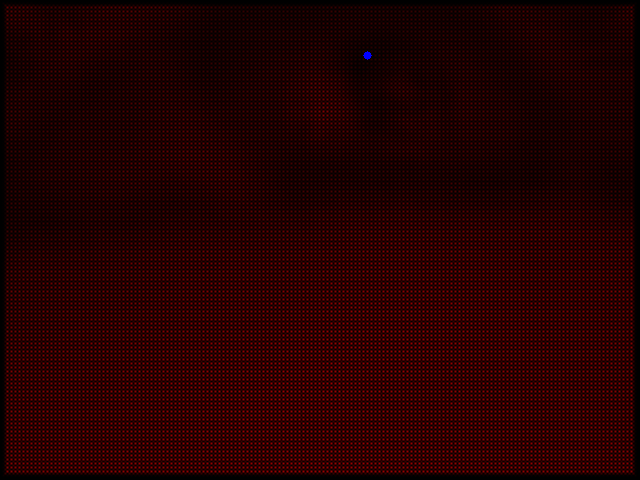
\includegraphics[width=0.9\linewidth]{plots/results/responsehaarbest.png}
        \caption{feature vector, blue is the best response}
    \end{subfigure}%
 
    \caption{Feature vector for pupil detection}
    \label{fig:limit_haar}
\end{figure}

The stronges response lies then within the pupil and the location is then used to create a ROI. In this case a ROI of $110 x 110$ was the norm but depending on the rescaling of the frames this can be adapted. Important to note is, that the returned point in the pupil is not given to be in the center. This in an important fact when choosing the size of the ROI that is created. 
But this approach is still not perfect and even though it can handle noise really good, there are limits to the amount of noise until the algorithm fails. Also the algorithm is not able to detect the pupil when the eye is closed.

\begin{figure}[h]
    \centering
    \begin{subfigure}{0.5\textwidth}
        \centering
        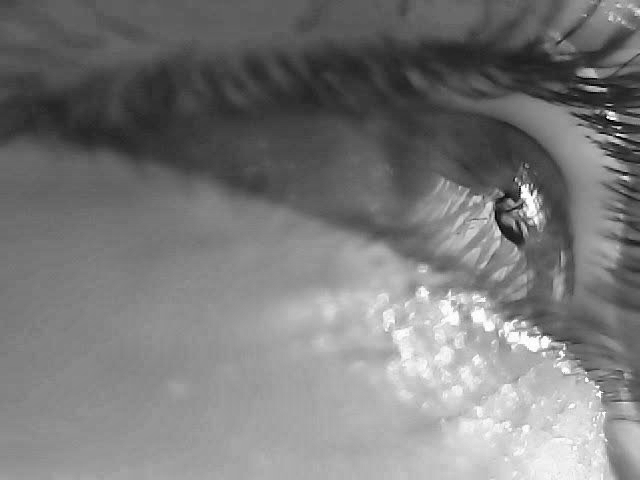
\includegraphics[width=0.9\linewidth]{plots/results/originalworst.png}
        \caption{Extreme noise example}
    \end{subfigure}%
    \hfill
    \begin{subfigure}{0.5\textwidth}
        \centering
        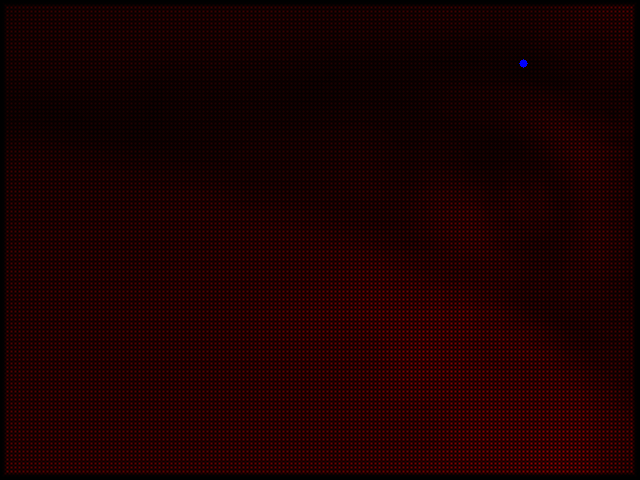
\includegraphics[width=0.9\linewidth]{plots/results/responsehaarworst.png}
        \caption{feature vector result with best response}
    \end{subfigure}%
 
    \caption{Limits to the Haar-like feature approach}
    \label{fig:limit_haar}
\end{figure}
The problem with the LPW data set is, that it is so versatile and the conditions change during the recording. This makes it hard to find an approach that can adapt to all the conditions and still perform well in a given time interval. The implementation can still be improved and sped up, in the Haar-like feature the following libraries were used to speed up the algorithm: 

\begin{python}
from concurrent.futures import ThreadPoolExecutor
from numba import njit
    \end{python}
ThreadPool Executor makes it possible to use multithreading and njit compiles the sliding window over the integral image of the Haar-like feature to machine code for more efficient calculation.

\section{Ellipse parameter estimation}
In the second part of an pupil detection algorithm it is necessary to make use of the informations from the first part and build on this foundation and find the five ellipse parameter: center: $(x,y)$, axis: (major, minor) and angle. The LPW has labels for the center only of the pupil and therefore only the center can be used to evaluate the performance of the algorithms. A second evaluation has to be done manually by inspecting the fit of the ellipse to the pupil. This is hard to evaluate with numerical methods and the result needs therefore to be taken with a grain of salt. In this section 4 different algorithms will be discussed and evaluated: The OpenCV ellipse fit based on contours (binary thresholding), ACWE with OpenCV Ellipse fit, ACWE combined with RANSAC, and Canny edge detection with OpenCV Ellipse fit. 

\subsection{Thresholding and OpenCV ellipse fit}
\label{}
The benefit of this method is that it can almost run in realtime and still perform well in certain frames where the noise is low and the pupil is clearly visible. But as already mentioned in the localization part, this method is not robust enough to handle the LPW data set. The thresholding is done with the same approach as in the localization part and the binary mask is then used to find the contours. The contours are then evaluated by their circularity and similarity to an ellipse. The best fitting contour is then used to fit an ellipse with the OpenCV ellipse fit function. The OpenCV ellipse fit function is based on the least square method and therefore very robust and fast. The ellipse fit is then evaluated by the center and the distance to the ground truth center. The problem with least square method is, lies in the definition itself. Because the method tries to find an ellipse that minimizes the distance from every point on the boundary of the binary mask to the ellipse curve. When the pupil is partially covered by noise, the contour does not match the original shape of the pupil and does not represent the total pupil boundary. Using least square method in this case leads to a faulty ellipse fit where the result is not usable. The amount of outliers is to high and the ellipse fit is not accurate enough because there is information missing. 
\begin{figure}[h]
    \centering
    \begin{subfigure}{0.3\textwidth}
        \centering
        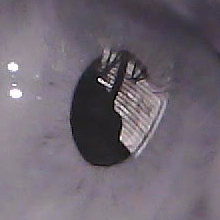
\includegraphics[width=0.9\linewidth]{plots/results/roi_text_resutls.png}
        \caption{ROI}
    \end{subfigure}%
    \hfill
    \begin{subfigure}{0.3\textwidth}
        \centering
        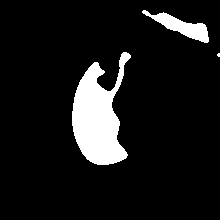
\includegraphics[width=0.9\linewidth]{plots/results/roi_binary_ellipse.png}
        \caption{Binary thresholding}
    \end{subfigure}%
    \hfill
    \begin{subfigure}{0.3\textwidth}
        \centering
        \includegraphics[width=0.9\linewidth]{plots/results/roi_result_binary_ellipse.png}
        \caption{OpenCV Ellipse fit}
    \end{subfigure}%
    \caption{Binary thresholding with OpenCV ellipse fit}
    \label{fig:binary_threshold_ellipse_fit}
\end{figure}

\subsection{Canny edge detection with OpenCV ellipse fit or RANSAC}
For this combination, the first step is to find the ROI, this is done with the Haar-like feature. This is from great importance because otherwise there is no chance in detecting the pupil boundary. The image is blured with a gaussian blur and after wards the Canny edge detection is used on it (Using the gradient, by calculating the sobel gradient). Afterwards the contours are found and evaluated by their circularity and similarity to an ellipse. The best matching contour is further processed with the OpenCV ellipse fit but the RANSAC is also an valid option. This results in the pupil boundary. The problem with this approach is, that the boundary needs to be clearly visible and the threshold values have to be choosen smart. Here the already known intensity value from the given point inside the pupil is used to make a decision for the thresholding values needed by the Canny edge detection. The benefit of this algorithm is the speed at which the frames can be processed. But overall this combination is not considered to be robust enough to handle the LPW data set and is therefore not further evaluated.

\subsection{ACWE with OpenCV ellipse fit}
This approach uses the OpenCV ellipse fit to interpret the results from the ACWE, the benefit is, that it runs faster than the RANSAC but it is strongly dependent on the quality of the binary mask returned by the ACWE. If the mask is not completely on the boundary of the pupil, the ellipse fit will also not fit the pupil because of the least square fit used in OpenCV ellipse fit.  ACWE andOpenCV ellipse fit works in low noise environment just as the thresholding approach. When comparing the threshold and contour segmentation with the ACWE with OpenCV ellipse fit, it can be seen that the quality of the approximation is almost the same. But in terms of speed ACWE with ellipse fit can not even be close to the thresholding approach. Especially when the pupil is large, the ACWE takes a long time to converge to the boundary of the pupil because ACWE can only enxtend for a certain amount each iteration whereas the thresholding finds the contour of the pupil in one iteration and a fraction of time compared to ACWE.


\subsection{ACWE combined with RANSAC}
\label{sus:acwe_ransac}
The benefit of using ACWE discussed in section \ref{sus:acwe}and the RANSAC method already discussed in section \ref{sus:ransac} is that the ellipse fit is not anymore based on least square method but instead uses a different approach as already introduced in the RANSAC section. This leads to a better fit but with the downsize of a increas in computational effort. This tradeoff is worth it when the images contain a lot of noise and the pupil boundary is not completly visible. If only a part of the boundary is visible, the accuracy of the ACWE combined with RANSAC is greater than when just using the OpenCV Ellipse fit. The RANSAC algorithm is applied to the binary mask returned by the ACWE that is created by an initial mask on a point taken from the Haar-like Feature detection. As already foreshadowed, the process contains a lot of steps and with ACWE being an iterative algorithm can take some time. The mask retrieved from ACWE is before using with the ransac algorithm dilated and eroded to remove small noise pixels and to make the mask smother. Only then the contour from the mask is used with the RANSAC algorithm. The RANSAC algorithm is applied on the contour points and tries to fit an ellipse to a random subset of the contour points. The approach to find the best ellipse uses this equation to evaluate the quality of the ellipse fit: 


\begin{gather}
    \text{InlierRatio} = \frac{n_{\text{inliers}}}{n_{\text{total\_points}}} \\
    \text{BorderRatio} = \frac{n_{\text{border}}}{n_{\text{total\_points}}} \\
    \text{Area} = \pi \cdot a \cdot b \\
    \text{Fit} = \alpha \cdot \text{InlierRatio} + \beta \cdot \text{BorderRatio} - \frac{\text{Area}}{n_{\text{total\_points}}} \cdot \pi
\end{gather}

with $\alpha = 100$, $\beta = 300$, $a$ and $b$ the major and minor aixs of the ellipse. The $InlierRatio$ is the ratio of inliers to the total number of points, the $BorderRatio$ is the ratio of points on the border of the ellipse to the total number of points and the Area is the area of the ellipse. The Fit is then calculated by a weighted sum of the $InlierRatio$, $BorderRatio$ and the $Area$. The weights are chosen by testing and are not optimal but work well enough and can be further adapted. 

In each iteration of the RANSAC the fit is calculated and if the current ellipse parameters have a greater fit than the previous ellipse parameters, if the fit is better, the current ellipse parameters are saved as the best fit. After $N$ iterations the best fit is returned as the approximation of the pupil ellipse. 

The reason for using a fit equation is that the individual conditions can exclude each other. When using a conditional logic the evaluation of a fit becomes tricky and strongly dependent on the order of the ellipses.  For example if the ellipse has a small area, which is considered as a good fit, but only $20\%$ of inliers it rejects all following ellipses based on the area. Therefore conditional logic is not considered for the evaluation of the ellipses. 
Here is an example fit in a very noise environment to show the robustness of the algorithm: 


\chapter{Proposal}
\label{chap:proposal}
\section{Proposed Algorithm}
After intensive research and analysis, the algorithm proposed for pupil detection consist of the following steps: 
\begin{enumerate}
    \item \textbf{Preprocessing:} The image is converted to grayscale and then histogram equalization method CLAHE is used to improve the contrast of the image.
    \item \textbf{Haar-like features:} From the image the feature vector is calculated using the Haar-like feature for pupil detection proposed by \cite{HaarLikeFeatures}. The feature vector is then used to find the strongest repsonse in the image. This point is considered to be inside the pupil area. 
    \item \textbf{ACWE} The active contour without edges algorithm is applied to the image with the point returned by the Haar-like features as center of the initial contour. Returns the contour of the pupil.
    \item \textbf{RANSAC} The RANSAC algorithm is applied to the mask returned by the ACWE algorithm. Iterates over the mask contour and fits a circle to a random subset of the contour points. Returns the circle with the highest number of inliers.
\end{enumerate}
\chapter{Results}
In this chapter the proposed algorithm is evaluated on the LPW data set and numerical results are presented, followed by a discussion of the results. 
\section{Evaluation}
\section{Discussion}
\section{Possible Improvements}

\chapter{Conclusion}
\label{chap:conclusion}
\section{Summary}
\label{sec:summary}
In this thesis, a diverse set of existing algorithms for pupil detection, each demonstrating its unique strengths and weaknesses, have been examined. These algorithms were analyzed under various imaging conditions, giving insight into their robustness and efficiency.

The Results show that finding a robust and efficient combination of algorithms is challenging and that the proposed algorithm cannot solve this task in real-time. The proposed algorithm presents a valid combination but still has weaknesses and needs adaptation to the specific use cases. The parameters must be repeatedly tuned on each data set and can not be seen as just working. The thesis aimed to evaluate and compare different algorithms and show their limitations, and this goal was achieved, and an overview of different approaches is given. The proposed algorithm can only be regarded as a solution that outperforms every method in some use cases.

Although the combination of Haar-like features, ACWE and RANSAC can perform well in even tricky conditions, there is still room for improvement and further research. Especially the Haar-like feature detection stood out with exceptional reliability for finding points inside the pupil and is considered the best method to gain information about the pupil's location.

The estimation of the pupil boundary with the proposed algorithm is valid but not perfect. The ellipse fit can still be improved by further tuning the parameters of the individual algorithms. The performance can be increased by implementing the code into C++ and using more multithreading and parallelization. It is unknown if the proposed algorithm can run in real time, but there is a high chance it is possible with further improvements. The estimation quality is sufficient to be used as a starting point for training a highly reliable AI-based eye Tracker or Iris recognition system and gaze tracing.  

The code published on GitHub can be used as a starting point to build more complex tasks on.  

%\chapter{Algorithms}

In this chapter will take a look at commonly used algorithms in image processing for edge detection, identifyig areas of interest and refining them. 
We discuss those algorithms first in theory and then show it's use case in detecting the iris of an human eye. 

To show the nature of the algorithm, the same preprocessed image is used and therefore it is possible to showcase the results and compare the algorithms in a later chapter
\section{Hough Transformation}

Dummy text.

\subsection{Definition Hough Transformation }

Dummy text.
$ 3/12$ 
\section{RANSAC}

Dummy text.

\subsection{Definition RANSAC}

Dummy text.


\section{Canny Edge Detection}

Dummy text.

\subsection{Definition Canny Edge Detection}

Dummy text.

\section{Active Contur}

Dummy text.

\subsection{Definition Active Countur}

Dummy text.

\subsubsection{Example Subsubsection}

Dummy text.

\paragraph{Example Paragraph}

Dummy text.

\subparagraph{Example Subparagraph}

Dummy text.

%\chapter{Writing scientific texts in English}

This chapter was originally a separate document written by Reto
Spöhel.  It is reprinted here so that the template can serve as a
quick guide to thesis writing, and to provide some more example
material to give you a feeling for good typesetting.

% We're going to need an extra theorem-like environment for this
% chapter
\theoremstyle{plain}
\theoremsymbol{}
\newtheorem{Rule}[theorem]{Rule}

\section{Basic writing rules}

The following rules need little further explanation; they are best
understood by looking at the example in the booklet by Knuth et al.,
§2--§3.

\begin{Rule}
  Write texts, not chains of formulas.
\end{Rule}

More specifically, write full sentences that are logically
interconnected by phrases like `Therefore', `However', `On the other
hand', etc.\ where appropriate.

\begin{Rule}
  Displayed formulas should be embedded in your text and punctuated
  with it.
\end{Rule}

In other words, your writing should not be divided into `text parts'
and `formula parts'; instead the formulas should be tied together by
your prose such that there is a natural flow to your writing.

\section{Being nice to the reader}

Try to write your text in such a way that a reader enjoys reading
it. That's of course a lofty goal, but nevertheless one you should
aspire to!

\begin{Rule}
  Be nice to the reader.
\end{Rule}

Give some intuition or easy example for definitions and theorems which
might be hard to digest. Remind the reader of notations you introduced
many pages ago -- chances are he has forgotten them. Illustrate your
writing with diagrams and pictures where this helps the reader. Etc.

\begin{Rule}
  Organize your writing.
\end{Rule}

Think carefully about how you subdivide your thesis into chapters,
sections, and possibly subsections.  Give overviews at the beginning
of your thesis and of each chapter, so the reader knows what to
expect. In proofs, outline the main ideas before going into technical
details. Give the reader the opportunity to `catch up with you' by
summing up your findings periodically.

\emph{Useful phrases:} `So far we have shown that \ldots', `It remains
to show that \ldots', `Recall that we want to prove inequality (7), as
this will allow us to deduce that \ldots', `Thus we can conclude that
\ldots. Next, we would like to find out whether \ldots', etc.

\begin{Rule}
  Don't say the same thing twice without telling the reader that you
  are saying it twice.
\end{Rule}

Repetition of key ideas is important and helpful. However, if you
present the same idea, definition or observation twice (in the same or
different words) without telling the reader, he will be looking for
something new where there is nothing new.

\emph{Useful phrases:} `Recall that [we have seen in Chapter 5 that]
\ldots', `As argued before / in the proof of Lemma 3, \ldots', `As
mentioned in the introduction, \ldots', `In other words, \ldots', etc.

\begin{Rule}
  Don't make statements that you will justify later without telling
  the reader that you will justify them later.
\end{Rule}

This rule also applies when the justification is coming right in the
next sentence!  The reasoning should be clear: if you violate it, the
reader will lose valuable time trying to figure out on his own what
you were going to explain to him anyway.

\emph{Useful phrases:} `Next we argue that \ldots', `As we shall see,
\ldots', `We will see in the next section that \ldots, etc.


\section{A few important grammar rules}

\begin{Rule}
  \label{rule:no-comma-before-that}
  There is (almost) \emph{never} a comma before `that'.
\end{Rule}

It's really that simple. Examples:
\begin{quote}
  We assume that \ldots\\
  \emph{Wir nehmen an, dass \ldots}

  It follows that \ldots\\
  \emph{Daraus folgt, dass \ldots}

  `thrice' is a word that is seldom used.\\
  \emph{`thrice' ist ein Wort, das selten verwendet wird.}
\end{quote}
Exceptions to this rule are rare and usually pretty obvious. For
example, you may end up with a comma before `that' because `i.e.' is
spelled out as `that is':
\begin{quote}
  For \(p(n)=\log n/n\) we have \ldots{} However, if we choose \(p\) a
  little bit higher, that is \(p(n)=(1+\varepsilon)\log n/n\) for some
  \(\varepsilon>0\), we obtain that\ldots
\end{quote}
Or you may get a comma before `that' because there is some additional
information inserted in the middle of your sentence:
\begin{quote}
  Thus we found a number, namely \(n_0\), that satisfies equation (13).
\end{quote}
If the additional information is left out, the sentence has no comma:
\begin{quote}
  Thus we found a number that satisfies equation (13).
\end{quote}
(For `that' as a relative pronoun, see also
Rules~\ref{rule:non-defining-has-comma}
and~\ref{rule:defining-without-comma} below.)

\begin{Rule}
  There is usually no comma before `if'.
\end{Rule}

Example:
\begin{quote}
  A graph is not \(3\)-colorable if it contains a \(4\)-clique.\\
  \emph{Ein Graph ist nicht \(3\)-färbbar, wenn er eine \(4\)-Clique
    enthält.}
\end{quote}
However, if the `if' clause comes first, it is usually separated from
the main clause by a comma:
\begin{quote}
  If a graph contains a \(4\)-clique, it is not \(3\)-colorable .\\
  \emph{Wenn ein Graph eine \(4\)-Clique enthält, ist er nicht
    \(3\)-färbbar.}
\end{quote}

There are more exceptions to these rules than to
Rule~\ref{rule:no-comma-before-that}, which is why we are not
discussing them here. Just keep in mind: don't put a comma before `if'
without good reason.

\begin{Rule}
  \label{rule:non-defining-has-comma}
  Non-defining relative clauses have commas.
\end{Rule}
\begin{Rule}
  \label{rule:defining-without-comma}
  Defining relative clauses have no commas.
\end{Rule}

In English, it is very important to distinguish between two types of
relative clauses: defining and non-defining ones. This is a
distinction you absolutely need to understand to write scientific
texts, because mistakes in this area actually distort the meaning of
your text!

It's probably easier to explain first what a \emph{non-defining}
relative clause is. A non-defining relative clauses simply gives
additional information \emph{that could also be left out} (or given in
a separate sentence). For example, the sentence
\begin{quote}
  The \textsc{WeirdSort} algorithm, which was found by the famous
  mathematician John Doe, is theoretically best possible but difficult
  to implement in practice.
\end{quote}
would be fully understandable if the relative clause were left out
completely. It could also be rephrased as two separate sentences:
\begin{quote}
  The \textsc{WeirdSort} algorithm is theoretically best possible but
  difficult to implement in practice. [By the way,] \textsc{WeirdSort}
  was found by the famous mathematician John Doe.
\end{quote}
This is what a non-defining relative clause is. \emph{Non-defining
  relative clauses are always written with commas.} As a corollary we
obtain that you cannot use `that' in non-defining relative clauses
(see Rule~\ref{rule:no-comma-before-that}!). It would be wrong to
write
\begin{quote}
  \st{The \textsc{WeirdSort} algorithm, that was found by the famous
    mathematician John Doe, is theoretically best possible but
    difficult to implement in practice.}
\end{quote}
A special case that warrants its own example is when `which' is
referring to the entire preceding sentence:
\begin{quote}
  Thus inequality (7) is true, which implies that the Riemann
  hypothesis holds.
\end{quote}
As before, this is a non-defining relative sentence (it could be left
out) and therefore needs a comma.

So let's discuss \emph{defining} relative clauses next. A defining
relative clause tells the reader \emph{which specific item the main
  clause is talking about}. Leaving it out either changes the meaning
of the sentence or renders it incomprehensible altogether.  Consider
the following example:

\begin{quote}
  The \textsc{WeirdSort} algorithm is difficult to implement in
  practice. In contrast, the algorithm that we suggest is very simple.
\end{quote}

Here the relative clause `that we suggest' cannot be left out -- the
remaining sentence would make no sense since the reader would not know
which algorithm it is talking about. This is what a defining relative
clause is. \textit{Defining relative clauses are never written with
  commas.} Usually, you can use both `that' and `which' in defining
relative clauses, although in many cases `that' sounds better.

As a final example, consider the following sentence:
\begin{quote}
  For the elements in \(\mathcal{B}\) which satisfy property (A), we
  know that equation (37) holds.
\end{quote}
This sentence does not make a statement about all elements in
\(\mathcal{B}\), only about those satisfying property (A). The relative
clause is \emph{defining}. (Thus we could also use `that' in place of
`which'.)

In contrast, if we add a comma the sentence reads
\begin{quote}
  For the elements in \(\mathcal{B}\), which satisfy property (A), we
  know that equation (37) holds.
\end{quote}

Now the relative clause is \emph{non-defining} -- it just mentions in
passing that all elements in \(\mathcal{B}\) satisfy property (A). The
main clause states that equation (37) holds for \emph{all} elements in
\(\mathcal{B}\). See the difference?


\section[Things you (usually) don't say in English]%
{Things you (usually) don't say in English -- and what to say
  instead}
\label{sec:list}

Table~\ref{tab:things-you-dont-say} lists some common mistakes and
alternatives.  The entries should not be taken as gospel -- they don't
necessarily mean that a given word or formulation is wrong under all
circumstances (obviously, this depends a lot on the context). However,
in nine out of ten instances the suggested alternative is the better
word to use.

\begin{table}
  \centering
  \caption{Things you (usually) don't say}
  \label{tab:things-you-dont-say}
  \begin{tabular}{lll}
    \toprule
    \st{It holds (that) \dots} & We have \dots & \emph{Es gilt \dots}\\
    \multicolumn{3}{l}{\quad\footnotesize(`Equation (5) holds.' is fine, though.)}\\
    \st{$x$ fulfills property $\mathcal{P}$.}& \(x\) satisfies property \(\mathcal{P}\). & \emph{\(x\) erfüllt Eigenschaft \(\mathcal{P}\).} \\
    \st{in average} & on average & \emph{im Durchschnitt}\\
    \st{estimation} & estimate   & \emph{Abschätzung}\\
    \st{composed number} & composite number & \emph{zusammengesetzte Zahl}\\
    \st{with the help of} & using & \emph{mit Hilfe von}\\
    \st{surely} & clearly & \emph{sicher, bestimmt}\\
    \st{monotonously increasing} & monotonically incr. & \emph{monoton steigend}\\
    \multicolumn{3}{l}{\quad\footnotesize(Actually, in most cases `increasing' is just fine.)}\\
    \bottomrule
  \end{tabular}
\end{table}

%%% Local Variables:
%%% mode: latex
%%% TeX-master: "thesis"
%%% End:

%\chapter{Typography}


\section{Punctuation}

\begin{Rule}
  Use opening (`) and closing (') quotation marks correctly.
\end{Rule}

In \LaTeX, the closing quotation mark is typed like a normal
apostrophe, while the opening quotation mark is typed using the French
\emph{accent grave} on your keyboard (the \emph{accent grave} is the
one going down, as in \emph{frère}).

Note that any punctuation that \emph{semantically} follows quoted
speech goes inside the quotes in American English, but outside in
Britain.  Also, Americans use double quotes first.  Oppose
\begin{quote}
  ``Using `lasers,' we punch a hole in \ldots\ the Ozone Layer,''
  Dr.\ Evil said.
\end{quote}
to
\begin{quote}
  `Using ``lasers'', we punch a hole in \ldots\ the Ozone Layer',
  Dr.\ Evil said.
\end{quote}

\begin{Rule}
  Use hyphens (-), en-dashes (--) and em-dashes (---) correctly.
\end{Rule}

A hyphen is only used in words like `well-known', `$3$-colorable'
etc., or to separate words that continue in the next line (which is
known as hyphenation).  It is entered as a single ASCII hyphen
character (\texttt{-}).

To denote ranges of numbers, chapters, etc., use an en-dash (entered
as two ASCII hyphens \texttt{--}) with no spaces on either side.  For
example, using Equations (1)--(3), we see\ldots

As the equivalent of the German \emph{Gedankenstrich}, use an en-dash
with spaces on both sides -- in the title of Section \ref{sec:list},
it would be wrong to use a hyphen instead of the dash. (Some English
authors use the even longer emdash (---) instead, which is typed as
three subsequent hyphens in \LaTeX. This emdash is used without spaces
around it---like so.)


\section{Spacing}

\begin{Rule}
  \label{rule:no-manual-spacing}
  Do not add spacing manually.
\end{Rule}

You should never use the commands \lstinline-\\- (except within
tabulars and arrays), \lstinline[showspaces=true]-\ - (except to
prevent a sentence-ending space after Dr.\ and such),
\lstinline-\vspace-, \lstinline-\hspace-, etc.  The choices programmed
into \LaTeX{} and this style should cover almost all cases.  Doing it
manually quickly leads to inconsistent spacing, which looks terrible.
Note that this list of commands is by no means conclusive.

\begin{Rule}
  Judiciously insert spacing in maths where it helps.
\end{Rule}

This directly contradicts Rule~\ref{rule:no-manual-spacing}, but in
some cases \TeX{} fails to correctly decide how much spacing is
required.  For example, consider
\begin{displaymath}
  f(a,b) = f(a+b, a-b).
\end{displaymath}
In such cases, inserting a thin math space \lstinline-\,- greatly
increases readability:
\begin{displaymath}
  f(a,b) = f(a+b,\, a-b).
\end{displaymath}

Along similar lines, there are variations of some symbols with
different spacing.  For example, Lagrange's Theorem states that
\(\abs{G}=[G:H]\abs{H}\), but the proof uses a bijection \(f\colon
aH\to bH\).  (Note how the first colon is symmetrically spaced, but
the second is not.)

\begin{Rule}
  Learn when to use \lstinline[showspaces=true]-\ - and
  \lstinline-\@-.
\end{Rule}

Unless you use `french spacing', the space at the end of a sentence is
slightly larger than the normal interword space.

The rule used by \TeX{} is that any space following a period,
exclamation mark or question mark is sentence-ending, except for
periods preceded by an upper-case letter.  Inserting \lstinline-\-
before a space turns it into an interword space, and inserting
\lstinline-\@- before a period makes it sentence-ending.  This means
you should write
\begin{lstlisting}
Prof.\ Dr.\ A. Steger is a member of CADMO\@.
If you want to write a thesis with her, you
should use this template.
\end{lstlisting}
which turns into
\begin{quote}
  Prof.\ Dr.\ A. Steger is a member of CADMO\@.  If you want to write
  a thesis with her, you should use this template.
\end{quote}
The effect becomes more dramatic in lines that are stretched slightly
during justification:
\begin{quote}
  \parbox{\linewidth}{\hbox to \linewidth{%
      Prof.\ Dr.\ A. Steger is a member of CADMO\@.  If you}}
\end{quote}

\begin{Rule}
  Place a non-breaking space (\lstinline-~-) right before references.
\end{Rule}

This is actually a slight simplification of the real rule, which
should invoke common sense.  Place non-breaking spaces where a line
break would look `funny' because it occurs right in the middle of a
construction, especially between a reference type (Chapter) and its
number.


\section{Choice of `fonts'}

Professional typography distinguishes many font attributes, such as
family, size, shape, and weight.  The choice for sectional divisions
and layout elements has been made, but you will still occasionally
want to switch to something else to get the reader's attention.  The
most important rule is very simple.

\begin{Rule}
  When emphasising a short bit of text, use \lstinline-\emph-.
\end{Rule}

In particular, \emph{never} use bold text (\lstinline-\textbf-).
Italics (or Roman type if used within italics) avoids distracting the
eye with the huge blobs of ink in the middle of the text that bold
text so quickly introduces.

Occasionally you will need more notation, for example, a consistent
typeface used to identify algorithms.

\begin{Rule}
  Vary one attribute at a time.
\end{Rule}

For example, for \textsc{WeirdSort} we only changed the shape to small
caps.  Changing two attributes, say, to bold small caps would be
excessive (\LaTeX{} does not even have this particular variation).
The same holds for mathematical notation: the reader can easily
distinguish \(g_n\), \(G(x)\), \(\mathcal{G}\) and \(\mathsf{G}\).

\begin{Rule}
  Never underline or uppercase.
\end{Rule}

No exceptions to this one, unless you are writing your thesis on a
typewriter.  Manually.  Uphill both ways.  In a blizzard.


\section{Displayed equations}

\begin{Rule}
  Insert paragraph breaks \emph{after} displays only where they
  belong.  Never insert paragraph breaks \emph{before} displays.
\end{Rule}

\LaTeX{} translates sequences of more than one linebreak (i.e., what
looks like an empty line in the source code) into a paragraph break in
almost all contexts.  This also happens before and after displays,
where extra spacing is inserted to give a visual indication of the
structure.  Adding a blank line in these places may look nice in the
sources, but compare the resulting display

\begin{displaymath}
  a = b
\end{displaymath}

to the following:
\begin{displaymath}
  a = b
\end{displaymath}
The first display is surrounded by blank lines, but the second is not.
It is bad style to start a paragraph with a display (you should always
tell the reader what the display means first), so the rule follows.

\begin{Rule}
  Never use \lstinline-eqnarray-.
\end{Rule}

It is at the root of most ill-spaced multiline displays.  The
\package{amsmath} package provides better alternatives, such as the
\lstinline-align- family
\begin{align*}
  f(x) &= \sin x, \\
  g(x) &= \cos x,
\end{align*}
and \lstinline-multline- which copes with excessively long equations:
\begin{multline*}
  \def\P{\mathrm P}
  \P\bigl[X_{t_0} \in (z_0, z_0+dz_0],\ldots, X_{t_n}\in(z_n,z_n+dz_n]\bigr]
  \\= \nu(dz_0) K_{t_1}(z_0,dz_1) K_{t_2-t_1}(z_1,dz_2)\cdots
  K_{t_n-t_{n-1}}(z_{n-1},dz_n).
\end{multline*}


\section{Floats}

By default this style provides floating environments for tables and
figures.  The general structure should be as follows:
\begin{lstlisting}
\begin{figure}
  \centering
  % content goes here
  \caption{A short caption}
  \label{some-short-label}
\end{figure}
\end{lstlisting}
Note that the label must follow the caption, otherwise the label will
refer to the surrounding section instead.  Also note that figures
should be captioned at the bottom, and tables at the top.

The whole point of floats is that they, well, \emph{float} to a place
where they fit without interrupting the text body.  This is a frequent
source of confusion and changes; please leave it as is.

\begin{Rule}
  Do not restrict float movement to only `here'
  \textnormal{(\lstinline-h-)}.
\end{Rule}

If you are still tempted, you should avoid the float altogether and
just show the figure or table inline, similar to a displayed equation.

%%% Local Variables:
%%% mode: latex
%%% TeX-master: "thesis"
%%% End:

%\chapter{Example Chapter}

Dummy text.

\section{Example Section}

Dummy text.

\subsection{Example Subsection}

Dummy text.

\subsubsection{Example Subsubsection}

Dummy text.

\paragraph{Example Paragraph}

Dummy text.

\subparagraph{Example Subparagraph}

Dummy text.


\appendix

\chapter{Dummy Appendix}

You can defer lengthy calculations that would otherwise only interrupt
the flow of your thesis to an appendix.


\backmatter

\bibliographystyle{unsrt}
\bibliography{refs}

\includepdf[pages={-}]{declaration-originality.pdf}

\end{document}
